\documentclass[../main.tex]{subfiles}

\begin{document}
While there exist datasets, such as \textsc{gamut}, useful for testing algorithms designed for finite games, we found no established projects for continuous games. To address this, we present a compilation of parametrized games drawn from both recent and classical literature, which should provide a convincing and comprehensive evaluation of any game-solving algorithm.

Note that continuous games are inherently complex, as even apparently simple games may only have Nash equilibria supported on infinitely many points. A case in point are \cref{ex.dresher61.pg111,ex.karlin59.vol2.sec71.ex2} played on the $[0,1]$ interval.

We chose to consistently present the utility function of player $i$ denoted as $u_i$ in the variables $x_{ij}$, where the first digit $i$ denotes the player, while $j$ is the variable index. None of the games that follow have more than ten players nor variables for any of the players.

\section{General Blotto}


The following examples are various settings for the classical two-player zero-sum game known as \emph{General Blotto}. The utility functions are sums of non-linearly weighted margins of victory over fronts.  \textcite{Golman2009} completely characterized the existence of pure equilibria for the following family of weighing functions:
\[
f(z) = \operatorname{sgn}(z)\,|z|^p
\]
parametrized by $p$, which is strictly positive for continuous games. The margins of victory are differences of products of the allocations to each front. 

\begin{example}\label{ex.golman09.isolated}
A two-player zero-sum game in $m \times m$ variables on the simplex
\[
x_i \in \Delta^{m-1} = \left\{ z \in \mathbb{R}^m \ \middle|\ z_j \ge 0,\ \sum_{j=1}^m z_j = 1 \right\} \quad \forall i \in \{1,2\}.
\]
The utility function is defined by
\[
u_1(x_1, x_2) = \sum_{j=1}^m f\left( x_{1j} - x_{2j} \right)
\]
where $f(x) = \operatorname{sign}(x)\,|x|^p$ and $p>0$. This is a continuous version of \emph{General Blotto}, where all isolated fronts have equal value. When $p = 1$, every strategy is optimal; when $p>1$, players may allocate all resources to any one front; no pure equilibrium exists for $p$ less than one \cite{Golman2009}.
\end{example}

\begin{example}\label{ex.golman09.pairs}
A two-player zero-sum game in $m \times m$ variables on the simplex
\[
x_i \in \Delta^{m-1} \quad \forall i \in \{1,2\}.
\]
The utility function is defined by
\[
u_1(x_1, x_2) = \sum_{i=1}^m\sum_{j=i+1}^m f\left( x_{1i}x_{1j} - x_{2i}x_{2j} \right) + \sum_{i=1}^m f\left( x_{1i} - x_{2i} \right)
\]
where $f(x) = \operatorname{sign}(x)\,|x|^p$ and $p>0$. This is a continuous version of \emph{General Blotto}, where all pairs of fronts have equal value. When $p = 1$, players should allocate $\frac{1}{m}$ to all fronts; otherwise, no pure equilibrium exists \cite{Golman2009}.
\end{example}

\begin{example}\label{ex.golman09.sets}
A two-player zero-sum game in $m \times m$ variables on the simplex
\[
x_i \in \Delta^{m-1} \quad \forall i \in \{1,2\}.
\]
The utility function is defined by
\[
u_1(x_1, x_2) = \sum_{\substack{I \subseteq \{1, \dots, m\} \\ I \ne \emptyset}} f\left( \prod_{i \in I} x_{1i} - \prod_{i \in I} x_{2i} \right)
\]
where $f(x) = \operatorname{sign}(x)\,|x|^p$ and $p>0$. This is a continuous version of \emph{General Blotto}, where all sets of fronts have equal value. When $p = 1$ players should allocate $\frac{1}{m}$ to all fronts. No pure equilibrium exists for other values of $p$ \cite{Golman2009}.
\end{example}

\section{Polynomial Saddle Point Games}
The following examples are the saddle point problems of polynomials studied by \textcite{nie.yang.ea:saddle}, which we have reinterpreted as two-player zero-sum polynomial games.

\begin{example}\label{ex.nie21.6.1.i}

A zero-sum 2-player polynomial game in $3 \times 3$ variables on the simplex
\[
x_i \in \Delta^{2} \quad \forall i \in \{1,2\}.
\]
The nonconcave-nonconvex utility function \cite[Example 6.1 (i)]{nie.yang.ea:saddle} is
\begin{align*}
u_{1}\left( x_{1}, x_{2} \right) &=  - x_{11} x_{12} - x_{11} x_{23} - x_{12} x_{13} - x_{13} x_{21} - x_{21} x_{22} - x_{22} x_{23}
\end{align*}
This game has the pure NE
\begin{align*}
x_1^\star \approx (0,1,0),\, x_2^\star \approx (0.25,0.5,0.25).
\end{align*}
\end{example}

\begin{example}\label{ex.nie21.6.1.ii}

A zero-sum 2-player polynomial game in $3 \times 3$ variables on the simplex
\[
x_i \in \Delta^{2} \quad \forall i \in \{1,2\}.
\]
The nonconcave-nonconvex utility function \cite[Example 6.1 (ii)]{nie.yang.ea:saddle} is
\begin{align*}
u_1(x_1, x_2) = &-x_{11}^3 - x_{12}^3 + x_{13}^3 + x_{21}^3 + x_{22}^3 - x_{23}^3 \\
    &- x_{13}x_{21}x_{22}(x_{21} + x_{22}) - x_{12}x_{21}x_{23}(x_{21} + x_{23}) - x_{11}x_{22}x_{23}(x_{22} + x_{23})
\end{align*}
This game has the pure NE
\begin{align*}
x_1^\star \approx (0,0,1),\, x_2^\star \approx (0,0,1).
\end{align*}
\end{example}


\begin{example}\label{ex.nie21.6.1.iii}

A zero-sum 2-player polynomial game in $4 \times 4$ variables on the simplex
\[
x_i \in \Delta^{3} \quad \forall i \in \{1,2\}.
\]
The nonconcave-nonconvex utility function \cite[Example 6.1 (iii)]{nie.yang.ea:saddle} is
\begin{align*}
u_{1}\left( x_{1}, x_{2} \right) &= \sum_{i=1}^{4} \sum_{\substack{j=1 \\ i \ne j}}^{4} (x_{1i} x_{1j} + x_{2i} x_{2j})  - \sum_{i=1}^{4} x_{1i}^2 x_{2i}^2 
\end{align*}
This game has 4 pure NE involving each one-hot vector $e_i$
\begin{align*}
\text{NE}_i:\;x_1^\star \approx (0.25,0.25,0.25,0.25),\, x_2^\star = e_i \quad \forall i \in \{1,2,3,4\}.
\end{align*}
\end{example}

\begin{example}\label{ex.nie21.6.1.iv}

A zero-sum 2-player polynomial game in $3 \times 3$ variables on the simplex
\[
x_i \in \Delta^{2} \quad \forall i \in \{1,2\}.
\]
the nonconcave-nonconvex utility function \cite[Example 6.1 (iv)]{nie.yang.ea:saddle} is
\begin{align*}
u_{1}\left( x_{1}, x_{2} \right) &= x_{23}^{2} x_{11}^{2} - x_{11} x_{12} x_{21} x_{22} - x_{11} x_{13} x_{21} x_{23} + x_{21}^{2} x_{12}^{2} - x_{12} x_{13} x_{22} x_{23} + x_{22}^{2} x_{13}^{2}
\end{align*}
The utility function has no saddle point.
\end{example}

\begin{example}\label{ex.nie21.6.2.i}

A zero-sum 2-player game in $2 \times 2$ variables on the unit hypercube
\[
x_i \in [0,1]^2 \quad \forall i \in \{1,2\}
\]
with the concave-nonconvex utility function
\begin{align*}
u_{1}\left( x_{1}, x_{2} \right) &=  - \left( 1 + x_{11} + x_{12} + x_{21} + x_{22} \right)^{2} + 4 \left( x_{11} + x_{22} + x_{11} x_{12} + x_{12} x_{21} + x_{21} x_{22} \right)
\end{align*}
\textcite[Example 6.2 (i)]{nie.yang.ea:saddle} report the pure NE
\begin{align*}
x_1^\star \approx (0.3249, 0.3249),\, x_2^\star = (1,0).
\end{align*}
Similarly, we recover a pure $\eps$-NE with any feasible $x_{11} = x_{12}$ and $x_2=(0,1)$.
\end{example}

\begin{example}\label{ex.nie21.6.2.ii}

A zero-sum 2-player game in $3 \times 3$ variables on the unit hypercube
\[
x_i \in [0,1]^3 \quad \forall i \in \{1,2\}
\]
with the nonconcave-nonconvex utility function \cite[Example 6.2 (ii)]{nie.yang.ea:saddle}
\begin{align*}
u_{1}\left( x_{1}, x_{2} \right) =  &- x_{11} - x_{12} - x_{13} - x_{21} - x_{22} - x_{23} - x_{22}^{2} x_{11}^{2} \\
&- x_{23}^{2} x_{11}^{2} + x_{21}^{2} x_{12}^{2} - x_{23}^{2} x_{12}^{2} + x_{21}^{2} x_{13}^{2} + x_{22}^{2} x_{13}^{2}
\end{align*}
The utility function has no saddle point.
\end{example}

\begin{example}\label{ex.nie21.6.3.i}

A zero-sum 2-player game in $3 \times 3$ variables on the hypercube
\[
x_i \in [-1,1]^3 \quad \forall i \in \{1,2\}
\]
with the nonconcave-nonconvex utility function \cite[Example 6.3 (i)]{nie.yang.ea:saddle}
\[
u_1(x_1, x_2) = -\sum_{i=1}^{3} (x_{1i} + x_{2i}) + \prod_{i=1}^{3} (x_{1i} - x_{2i})
\]
This game has three pure Nash equilibria:
\begin{align*}
\text{NE}_1: &x_1^\star = (−1, −1, 1), x_2^\star = (1, 1, 1),\\
\text{NE}_2: &x_1^\star = (−1, 1, −1), x_2^\star = (1, 1, 1),\\
\text{NE}_3: &x_1^\star = (1, −1, −1), x_2^\star = (1, 1, 1).
\end{align*}
\end{example}


\begin{example}\label{ex.nie21.6.3.ii}

A zero-sum 2-player game in $3 \times 3$ variables on the hypercube
\[
x_i \in [-1,1]^3 \quad \forall i \in \{1,2\}
\]
with the nonconcave-nonconvex utility function \cite[Example 6.3 (ii)]{nie.yang.ea:saddle}
\[
u_1(x_1, x_2) = -\sum_{i=1}^{3} x_{2i}^2 + \sum_{i=1}^{3} x_{1i}^2 - \sum_{\substack{i=1 \\ i < j}}^{3} \sum_{j=1}^{3} (x_{1i}x_{2j} - x_{1j}x_{2i})
\]
This game has the following pure Nash equilibrium:
\begin{align*}
x_1^\star = (-1, 1, −1), x_2^\star = (-1, 1, -1).
\end{align*}
\end{example}

\begin{example}\label{ex.nie21.6.4.i}

A zero-sum 2-player game in $3 \times 3$ variables on the sphere
\[
x_i \in \left\{ z \in \mathbb{R}^3 \,\middle|\, \norm{z} = 1  \right\} \quad \forall i \in \{1,2\}
\]
with the utility function \cite[Example 6.4 (i)]{nie.yang.ea:saddle}
\begin{align*}
u_1(x_1, x_2) = &-x_{11}^3 - x_{12}^3 - x_{13}^3 - x_{21}^3 - x_{22}^3 - x_{23}^3 \\
    &- 2(x_{11}x_{12}x_{21}x_{22} + x_{11}x_{13}x_{21}x_{23} + x_{12}x_{13}x_{22}x_{23})
\end{align*}
This game has the following 9 pure NE:
\begin{align*}
\text{NE}_{ij}:\;x_1^\star = e_i,\, x_2^\star = e_j \quad \forall i,j \in \{1,2,3\}.
\end{align*}
\end{example}


\begin{example}\label{ex.nie21.6.4.ii}

A zero-sum 2-player game in $3 \times 3$ variables on the sphere
\[
x_i \in \left\{ z \in \mathbb{R}^3 \,\middle|\, \norm{z} = 1  \right\} \quad \forall i \in \{1,2\}
\]
with the utility function \cite[Example 6.4 (ii)]{nie.yang.ea:saddle}
\begin{align*}
u_1(x_1, x_2) = &-x_{11}^2x_{21}^2 - x_{12}^2x_{22}^2 - x_{13}^2x_{23}^2 - x_{11}^2x_{22}x_{23} - x_{12}^2x_{21}x_{23} \\
    &- x_{13}^2x_{21}x_{22} - x_{21}^2x_{12}x_{13} - x_{22}^2x_{11}x_{13} - x_{23}^2x_{11}x_{12}
\end{align*}
The utility function has no saddle points.
\end{example}


\begin{example}\label{ex.nie21.6.5}

A zero-sum 2-player game in $3 \times 3$ variables on the ball
\[
x_i \in \left\{ z \in \mathbb{R}^3 \,\middle|\, \norm{z} \leq 1  \right\} \quad \forall i \in \{1,2\}
\]
with the nonconcave-convex utility function \cite[Example 6.5]{nie.yang.ea:saddle}
\[
u_1(x_1, x_2) = -x_{11}^2x_{21} - 2x_{12}^2x_{22} - 3x_{13}^2x_{23} + x_{11} + x_{12} + x_{13}
\]
This game has the following pure Nash equilibrium:
\begin{align*}
\text{NE}_3: &x_1^\star \approx (0.7264, 0.4576, 0.3492), x_2^\star \approx (0.6883, 0.5463, 0.4772).
\end{align*}
\end{example}

\begin{example}\label{ex.nie21.6.6}

A zero-sum 2-player game in $3 \times 3$ variables on the intersection of the nonnegative orthant and the sphere
\[
x_i \in \left\{ z \in \mathbb{R}^3_+ \,\middle|\, \norm{z} = 1  \right\} \quad \forall i \in \{1,2\}
\]
with the utility function \cite[Example 6.6]{nie.yang.ea:saddle}
\[
u_1(x_1, x_2) = -x_{11}^2x_{22}x_{23} - x_{21}^2x_{12}x_{13} - x_{12}^2x_{21}x_{23} - x_{22}^2x_{11}x_{13} - x_{13}^2x_{21}x_{22} - x_{23}^2x_{11}x_{12}
\]
The utility function has no saddle points.
\end{example}

\begin{example}\label{ex.nie21.6.10}

A zero-sum 2-player game in $5 \times 5$ variables on the simplex
\[
x_i \in \Delta^{4} \quad \forall i \in \{1,2\}.
\]
The utility function is defined by \cite[Example 6.10]{nie.yang.ea:saddle}
\[
u_1(x_1, x_2) = x_1^\top A_1 x_1 + x_2^\top A_2 x_2 + x_1^\top B x_2
\]
where the matrix parameters $A_1$, $A_2$, and $B$ are
\[
A_1 = \begin{bmatrix*}[r]
-4 & 4 & 0 & 3 & -4 \\
3 & 4 & 3 & -4 & -5 \\
-3 & 0 & -2 & 0 & 4 \\
-4 & -4 & -1 & 3 & -5 \\
4 & 1 & -3 & 0 & -5
\end{bmatrix*},\, A_2 = \begin{bmatrix*}[r]
-4 & 4 & 1 & 0 & 1 \\
-2 & -4 & 2 & -3 & 1 \\
-3 & 1 & 1 & 4 & 4 \\
3 & -4 & 0 & 1 & -2 \\
-1 & -3 & -1 & 3 & -2
\end{bmatrix*}
\]

\[
B = \begin{bmatrix*}[r]
-2 & -4 & -2 & -5 & 3 \\
0 & 0 & 2 & 4 & 2 \\
0 & -4 & -1 & -5 & 3 \\
1 & -3 & -4 & 0 & -3 \\
3 & -1 & -5 & 4 & -4
\end{bmatrix*}
\]
The game has the following two NE:
\begin{align*}
    \text{NE}_1: &x_1^\star = (0, 1, 0, 0, 0), x_2^\star = (1, 0, 0, 0, 0),\\
    \text{NE}_2: &x_1^\star = (0, 1, 0, 0, 0), x_2^\star = (0, 1, 0, 0, 0).
\end{align*}
\end{example}

\section{Miscellaneous Games}
The following is a list of example games appearing in papers and books by various authors, which we loosely grouped by the research topic.
\subsection{Games from Classical Literature}
The following games appear in books from the $1950$s and $60$s, where they were used as demonstrations that the solutions of continuous games may be supported on anything from singleton sets to Cantor sets and whole intervals.

\begin{game}\label{ex.dresher61.pg110}
A two-player zero-sum game in $1 \times 1$ variables on the interval
$$x_{i1} \in [0,1] \quad \forall i \in \{1, 2\},$$
with the utility function \cite[pg. 110]{Dresher2007-ez}
\begin{equation*}
u_{1}\left( x_{1}, x_{2} \right) = \left( x_{11} - x_{21} \right)^{2}
\end{equation*}
The Nash equilibrium is $\mu_1^\star = \mathcal{U}\{0,1\}$; $\mu_2^\star = \delta_{0.5}$ and the value is $\frac{1}{4}$.
\end{game}

\noindent
\begin{minipage}[c]{0.6\textwidth}
\begin{game}\label{ex.dresher61.pg111}
A two-player zero-sum game in $1 \times 1$ variables on the interval
$$x_{i1} \in [0,1] \quad \forall i \in \{1, 2\},$$
with the utility function
\begin{align*}
u_{1}\left( x_{1}, x_{2} \right) &= \left( 1 - \left| x_{21} - x_{11} \right| \right) \left|  x_{21} - x_{11} \right|
\end{align*}
\textcite[pg. 111]{Dresher2007-ez} proved that the only equilibrium of this game has an infinite support: $\mu_i^\star = \mathcal{U}[0,1]$, and its value is $\frac{1}{6}$.
\end{game}
\end{minipage}
\hfill
\begin{minipage}[c]{0.35\textwidth}
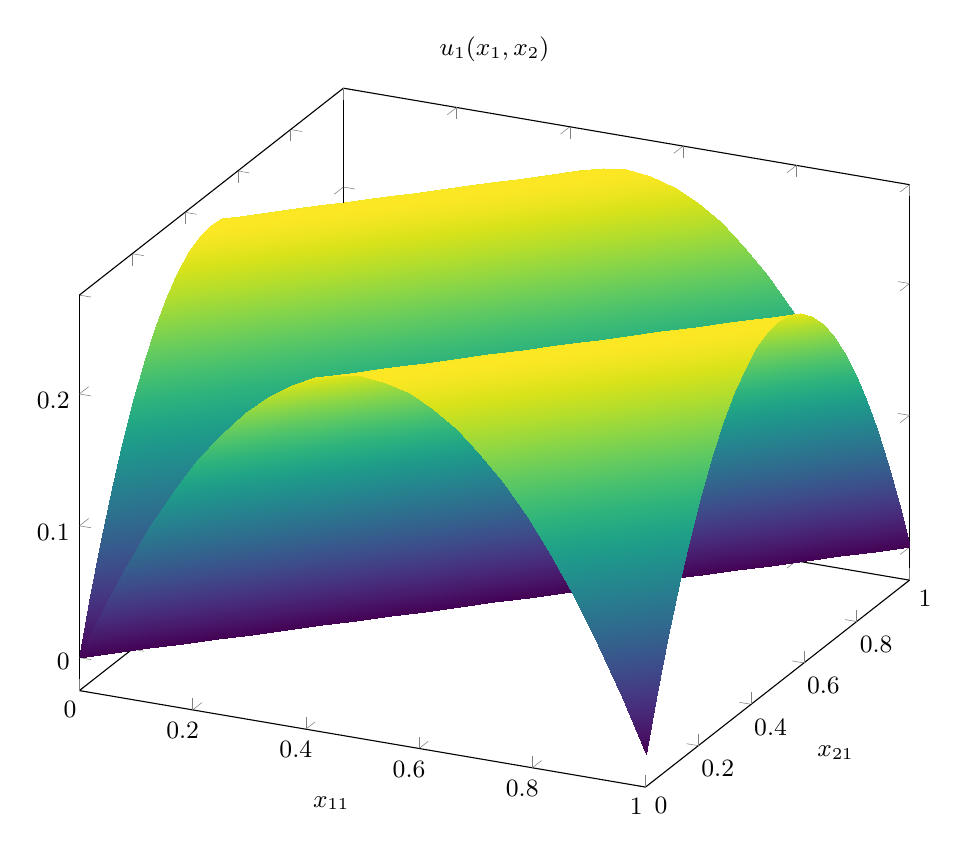
\begin{tikzpicture}
\begin{axis}[
    font=\small,
    domain=0:1,
    y domain=0:1,
    xlabel=$x_{11}$,
    ylabel=$x_{21}$,
    title={$u_1(x_1,x_2)$},
    colormap/viridis,
    mesh/ordering=y varies,
    width=\textwidth,
]
\addplot3[
    surf,
    shader=interp,
]
{abs(y - x) * (1 - abs(y - x))};
\end{axis}
\end{tikzpicture}
\end{minipage}


\begin{game} \label{ex.gross58.poly}
A two-player zero-sum game in $m_1 \times m_2$ variables on compact subsets of real numbers
\[
    x_i \in X_i \subset \mathbb{R}^{m_i} \quad \forall i \in \{1,2\}.
\]
The polynomial utility function is defined by
\begin{align*}
u(x_1,x_2)
= &f(x_1)ϕ(x_1) \left(g(x_2)ϕ(x_1) + \sum_{i=1}^{c_2} (g_i(x_2) - \mu_{2i}) ϕ_i(x_1) \right) \\
- &g(x_2)ψ(x_2) \left(f(x_1)ψ(x_2) + \sum_{i=1}^{c_1} (f_i(x_1) - \mu_{1i}) ψ_i(x_2) \right) \\
- &(f(x_1)ϕ(x_1))^2 + (g(x_2)ψ(x_2))^2
\end{align*}
where
\begin{align*}
f(x_1) &= \prod_{\substack{s \in \sigma_1}} \norm{x_1 - s}^2, &\phi(x_1) &= \prod_{\substack{a \in \alpha_1}} \norm{x_1 - a}^2,\\
f_i(x_1) &= \prod_{\substack{s \in \sigma_1 \\ s \neq \sigma_{1i}}} \frac{\norm{z-s}^2}{\norm{\sigma_{1i}-s}^2},&\phi_i(x_1) &= \prod_{\substack{a \in \alpha_1 \\ a \neq \alpha_{1i}}} \norm{x_1-a}^2;
\end{align*}
with $g$ and $\psi$ being defined analogously for $x_2$, $\sigma_2$, $\mu_2$, and $\alpha_2$.

This game has the property that the parameters $\sigma$ and $\mu$ define a unique mixed Nash equilibrium supported on $\sigma_i \in X_i^{c_i}$ weighted by $\mu_i \in \Delta^{c_i-1}$, for any set of cluster points $\alpha_i \in X_i^{c_{-i}+1}$ that do not overlap with the supports.

This construction of polynomial games with a unique prescribed solution was discovered by \textcite{gale1958note}. The generated games may be challenging to solve numerically given their large degrees and relative flatness near the equilibrium as shown in figure \ref{fig:gross}.
\end{game}

\begin{figure}
\centering
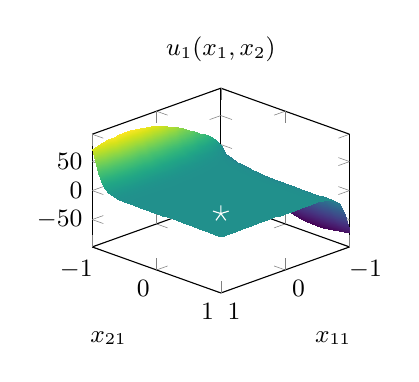
\begin{tikzpicture}
\begin{axis}[
    font=\small,
    domain=-1:1,
    y domain=-1:1,
    xlabel=$x_{11}$,
    ylabel=$x_{21}$,
    title={$u_1(x_1,x_2)$},
    colormap/viridis,
    view={135}{30},
    mesh/ordering=y varies,
    width=0.4\textwidth,
]
\addplot3[
    surf,
    shader=interp,
]
{-0.25*y^5 + 0.25*x*y^4 - 0.25*x^4*y + 0.25*x^5 + 2.25*y^6 - 2.0*x*y^5 - 0.25*x^2*y^4 + 0.25*x^4*y^2 + 2.0*x^5*y - 2.25*x^6 - 8.5*y^7 + 6.5*x*y^6 + 2.0*x^2*y^5 - 2.0*x^5*y^2 - 6.5*x^6*y + 8.5*x^7 + 17.5*y^8 - 11.0*x*y^7 - 6.5*x^2*y^6 + 6.5*x^6*y^2 + 11.0*x^7*y - 17.5*x^8 - 21.25*y^9 + 10.25*x*y^8 + 11.0*x^2*y^7 - 11.0*x^7*y^2 - 10.25*x^8*y + 21.25*x^9 + 15.25*y^10 - 5.0*x*y^9 - 10.25*x^2*y^8 + 10.25*x^8*y^2 + 5.0*x^9*y - 15.25*x^10 - 6.0*y^11 + x*y^10 + 5.0*x^2*y^9 - 5.0*x^9*y^2 - x^10*y + 6.0*x^11 + y^12 - x^2*y^10 + x^10*y^2 - x^12};
\addplot3[
    only marks,
    mark=star,
    color=white,
    mark size=3,
]
coordinates {(0.5, 0.5, 0)};
\end{axis}
\end{tikzpicture}
\caption{12-degree polynomial game on a hypercube with a prescribed solution at $0.5, 0.5$ constructed using the method described by \textcite{gale1958note}  with parameters $\alpha_i = (1, 0)$, $\sigma_i = (0.5)$, and $\mu_i = (1) \quad \forall i \in \{1,2\}$.}
\label{fig:gross}
\end{figure}

\begin{game}\label{ex.karlin59.vol2.sec71.ex1}
A two-player zero-sum game in $1 \times 1$ variables on the interval
$$x_{i1} \in [0,1] \quad \forall i \in \{1,2\}.$$
The utility function is defined by
\begin{equation*}
u_{1}\left( x_{1}, x_{2} \right) = \frac{1}{1 + \lambda \left( x_{11} - x_{21} \right)^{2}}
\end{equation*}
where $\lambda > 0$. \textcite[Example~1]{karlin:chapter} proved that the game has finitely supported optimal strategies.
\end{game}


\noindent
\begin{minipage}[c]{0.6\textwidth}
\begin{game}\label{ex.karlin59.vol2.sec71.ex2}
A two-player zero-sum game in $1 \times 1$ variables on the interval
$$x_{i1} \in [0,1] \quad \forall i \in \{1,2\}.$$
The utility is defined by the rational function
\begin{align*}
u_{1}\left( x_{1}, x_{2} \right) &=  \left( x_{21} - 0.5 \right)\left(\frac{1 + \left( x_{21} - 0.5 \right)^{2} \left( x_{11} - 0.5 \right)}{1 + \left( x_{21} - 0.5 \right)^{4} \left( x_{11} - 0.5 \right)^{2}} \right) \\
& - \frac{x_{21} - 0.5 }{1 + \left( x_{21} - 0.5 \right)^{4} \left( \frac{1}{3} x_{11} -0.5\right)}
\end{align*}
\textcite[Example~2]{karlin:chapter} proved that the unique optimal strategy is the Cantor distribution.
\end{game}
\strut
\end{minipage}
\hfill
\begin{minipage}[c]{0.35\textwidth}
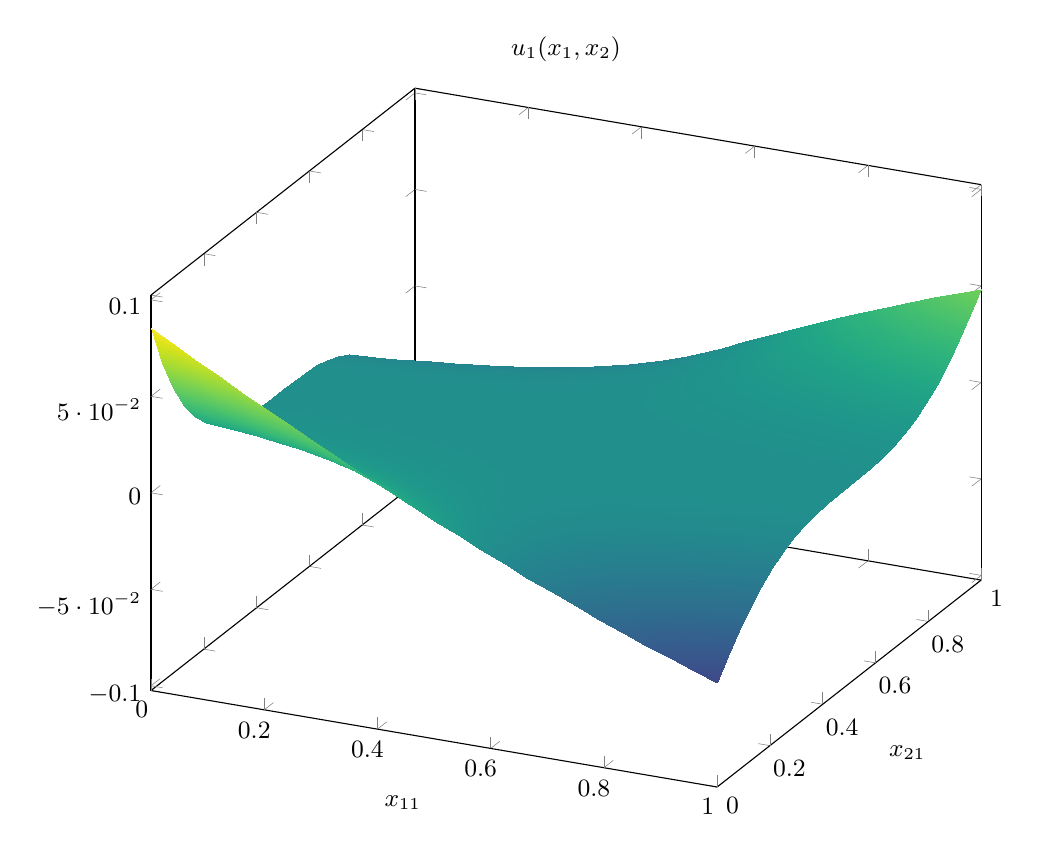
\begin{tikzpicture}
\begin{axis}[
    font=\small,
    domain=0:1,
    y domain=0:1,
    xlabel=$x_{11}$,
    ylabel=$x_{21}$,
    title={$u_1(x_1,x_2)$},
    colormap/viridis,
    mesh/ordering=y varies,
    width=\textwidth,
]
\addplot3[
    surf,
    shader=interp,
]
{(y - 0.5) * ((1 + (x - 0.5) * (y - 0.5)^2) / (1 + (x - 0.5)^2 * (y - 0.5)^4) - 1 / (1 + (x / 3 - 0.5) * (y - 0.5)^4))};
\end{axis}
\end{tikzpicture}
\end{minipage}


\begin{game}\label{ex.karlin59.vol2.sec76.pr1}
A two-player zero-sum game in $1 \times 1$ variables on the interval
$$x_{i1} \in [0,1] \quad \forall i \in \{1,2\}.$$
The utility is defined by \cite[Problem 1]{karlin:chapter}:
\begin{equation*}
u_{1}\left( x_{1}, x_{2} \right) = \frac{2 \left( x_{11} + x_{21} \right)}{\left( 1 + 2 x_{11} \right) \left( 1 + 2 x_{21} \right)}
\end{equation*}
The game has a Nash equilibrium where both players play $\mu^\star(z)=\frac{1+2z}{2}$.
\end{game}


\begin{game}\label{ex.karlin59.vol2.sec76.pr2}
A two-player zero-sum game in $1 \times 1$ variables on the interval
$$x_{i1} \in [0,1] \quad \forall i \in \{1,2\}.$$
The utility is defined by
\begin{equation*}
u_{1}\left( x_{1}, x_{2} \right) = \frac{\left( 1 + x_{11} \right) \left( 1 + x_{21} \right)}{\left( 1 + x_{11} x_{21} \right)^{2}}
\end{equation*}
\textcite[Problem 2]{karlin:chapter} showed that the value of this game is $\frac{1}{\ln 2}$ when both players play $\mu^\star(z)=\frac{\ln (1+z)}{\ln 2}$.

\end{game}


\subsection{Experiments on Games with Interesting Weaker Solution Concepts}


The following examples are from papers that study algorithms recovering weaker solution concepts, such as min-max critical points, due to the potential non-existence and the complexity of computing Nash Equilibria. Examples ... were used to demonstrate the failure of convergence of gradient-based algorithms.

\begin{game}\label{ex.daskalakis.d}
A two-player zero-sum game in $1 \times 1$ variables on the interval
$$x_{i1} \in [0,1] \quad \forall i \in \{1, 2\},$$
with the utility function
\begin{align*}
u_{1}\left( x_{1}, x_{2} \right) &= \left( -0.5 + x_{11} \right) \left( -0.5 + x_{21} \right).
\end{align*}
This game was studied by \textcite[Appendix D]{daskalakis.golowich.ea:stay-on-the-ridge}. The game has a value of $0$ and a pure Nash equilibrium at $(x_{11},x_{21}) = (0.5, 0.5)$.
\end{game}

\begin{game}\label{ex.daskalakis.e.1st}
A two-player zero-sum game in $1 \times 1$ variables on the interval
$$x_{i1} \in [0,1] \quad \forall i \in \{1, 2\},$$
with the utility function \cite[Appendix E]{daskalakis.golowich.ea:stay-on-the-ridge}
\begin{align*}
u_{1}\left( x_{1}, x_{2} \right) &= \left(  - 4 x_{11}^{2} + \frac{x_{21}^{4}}{10} + \left(  - 3 x_{11} + x_{21} + \frac{x_{11}^{3}}{20} \right)^{2} \right) e^{\frac{1}{100} \left(  - x_{11}^{2} - x_{21}^{2} \right)}
\end{align*}
The only local min-max equilibrium is $(x_{11},x_{21}) = (0, 0)$. This game was also studied by \textcite{Chinchilla2024,wang2019solvingminimaxoptimizationlocally,zheng.zhu.ea:universal}.
\end{game}


\begin{game}\label{ex.mertikopoulos18.fig1}
A two-player zero-sum game in $1 \times 1$ variables on the interval
$$x_{i1} \in [0,1] \quad \forall i \in \{1,2\}.$$
The utility function is defined by
\begin{align*}
u_{1}\left( x_{1}, x_{2} \right) &= -\left(x_{11}-\frac{1}{2}\right)\left(x_{21}-\frac{1}{2}\right)-\frac{1}{3}e^{-\left(x_{11}-\frac{1}{4}\right)^2-\left(x_{21}-\frac{3}{4}\right)^2}
\end{align*}
\textcite[Fig. 1]{mertikopoulos.lecouat.ea:optimistic} demonstrated divergent behavior of \emph{Mirror Descent} on this non-monotone saddle-point problem. The game has an $\eps$-NE:
\begin{align*}
\mu_1^\star &\approx \delta_{0.38},\\
\mu_2^\star &\approx 0.433\delta_{0} + 0.567\delta_{1}
\end{align*}
achieving a value of $0.247$.
\end{game}

\begin{game}\label{ex.mertikopoulos18.2.2}
A two-player zero-sum game in $1 \times 1$ variables on the interval
$$x_{i1} \in [-1,1] \quad \forall i \in \{1,2\}.$$
The utility function is
\begin{align*}
u_{1}\left( x_{1}, x_{2} \right) = \left( 1 - x_{21}^{2} + x_{21}^{4} x_{11}^{2} \right) \left( -1 - x_{11}^{2} - x_{21}^{2} x_{11}^{4} \right)
\end{align*}
This non-monotone saddle-point problem was studied by \textcite[(2.2)]{mertikopoulos.lecouat.ea:optimistic}. The unique saddle point is $x^\star = (0,0)$.
\end{game}


\noindent
\begin{minipage}[c]{0.6\textwidth}
\begin{game}\label{ex.razaviyayn20.5.1}
A two-player zero-sum game in $1 \times 1$ variables on the intervals
\begin{align*}
    x_1 &\in [-1,1]\\
    x_2 &\in [-2\pi, 2\pi]
\end{align*}
with the utility function \cite[Example~1]{razaviyayn.huang.ea:nonconvex}
\begin{align*}
u_{1}\left( x_{1}, x_{2} \right) &=  - \cos\left( x_{21} \right) + 0.2 x_{11} x_{21}
\end{align*}
The game has the $\epsilon$-NE:
\begin{align*}
\mu_1^\star &= 0.5\delta_{ -1 } + 0.5\delta_{ 1 }, \\
\mu_2^\star &= 0.5\delta_{ -2\pi } + 0.5\delta_{ 2\pi }.
\end{align*}

\end{game}
\strut
\end{minipage}
\hfill
\begin{minipage}[c]{0.35\textwidth}
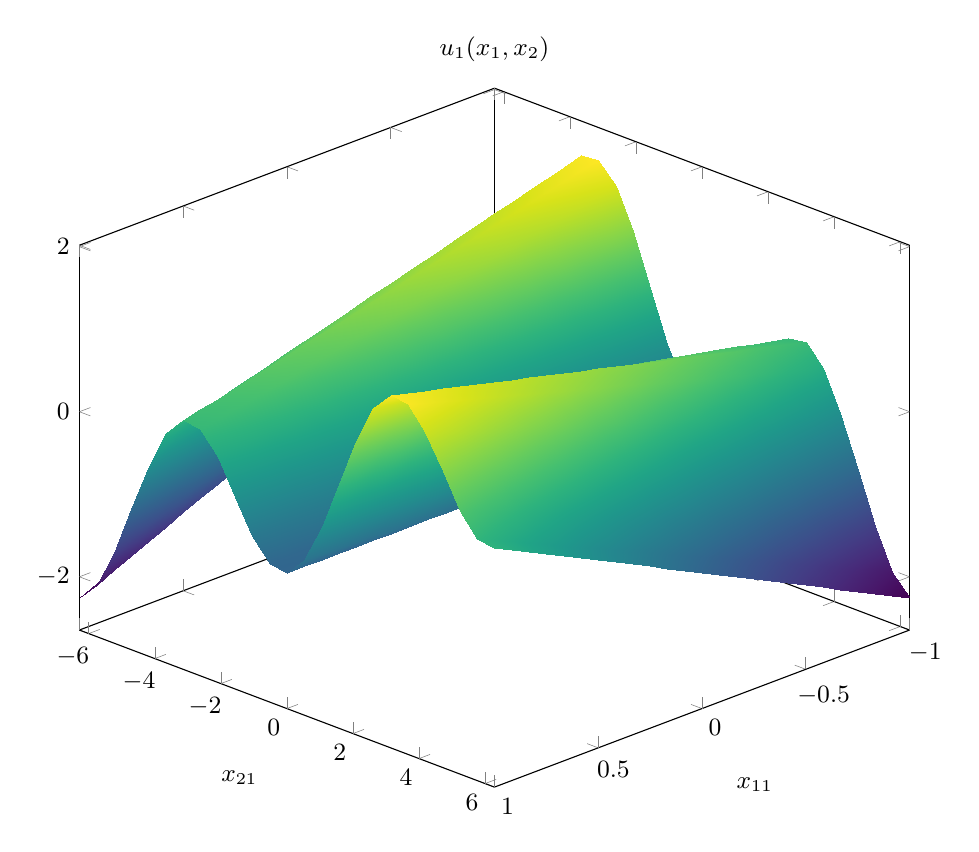
\begin{tikzpicture}
\begin{axis}[
    font=\small,
    domain=-1:1,
    y domain=-6.28318:6.28318,
    xlabel=$x_{11}$,
    ylabel=$x_{21}$,
    title={$u_1(x_1,x_2)$},
    colormap/viridis,
    view={135}{30},
    mesh/ordering=y varies,
    width=\textwidth,
]
\addplot3[
    surf,
    shader=interp,
]
{-cos(deg(y))+0.2*x*y};
\end{axis}
\end{tikzpicture}
\end{minipage}

\begin{game}\label{ex.razaviyayn20.5.3}
A two-player zero-sum game in $1 \times 1$ variables on the interval
\begin{align*}
    x_i &\in [-1,1] \quad \forall i \in \{1,2\}
\end{align*}
with the utility function \cite[Example~3]{razaviyayn.huang.ea:nonconvex}
\begin{align*}
u_{1}\left( x_{1}, x_{2} \right) &= 2 x_{11} x_{21} - x_{21}^{2} + x_{11}^{3}
\end{align*}
The game has the mixed $\epsilon$-NE:
\begin{align*}
\mu_1^\star &\approx \frac{1}{3}\delta_{1} + \frac{2}{3}\delta_{-0.5}, \\
\mu_2^\star &\approx \frac{5}{16}\delta_{1} + \frac{11}{16}\delta_{-1}.
\end{align*}
\end{game}

\begin{game}\label{ex.zheng23.convex.nonconcave}
A two-player zero-sum game in $1 \times 1$ variables on the interval
\begin{align*}
    x_i &\in [-1,1] \quad \forall i \in \{1,2\}
\end{align*}
with utility function given by
\begin{align*}
u_{1}\left( x_{1}, x_{2} \right) &=  - 2 x_{11}^{2} - 4 x_{11} x_{21} + x_{21}^{2} - \frac{4}{3} x_{21}^{3} + \frac{1}{4} x_{21}^{4}
\end{align*}
This example was studied by \textcite[Convex-Nonconcave Example]{zheng.zhu.ea:universal} and also \textcite{Chinchilla2024, pmlr-v89-adolphs19a}.
\end{game}

\begin{game}\label{ex.zheng23.kl.nonconcave}
A two-player zero-sum game in $1 \times 1$ variables on the interval
\begin{align*}
    x_i &\in [-1,1] \quad \forall i \in \{1,2\}
\end{align*}
with utility function \cite[KŁ-Nonconcave Example]{zheng.zhu.ea:universal} given by
\begin{align*}
u_{1}\left( x_{1}, x_{2} \right) &=  - x_{11}^{2} + 4 x_{21}^{2} + 10 \sin^{2}\left( x_{21} \right) - 3 \sin^{2}\left( x_{21} \right) \sin^{2}\left( x_{11} \right)
\end{align*}
This game has the pure NE $x^\star=(0,0)$.
\end{game}

\begin{game}\label{ex.zheng23.bilinearly.coupled.minimax}
A two-player zero-sum game in $1 \times 1$ variables on the interval
\begin{align*}
    x_i &\in [-4,4] \quad \forall i \in \{1,2\}
\end{align*}
with utility function \cite[Bilinearly-coupled Minimax]{zheng.zhu.ea:universal} given by
\begin{align*}
u_1(x_1, x_2) = - f(x_{11}) - Ax_{11}x_{21} + f(x_{21})
\end{align*}
where $f(z)=(z + 1)(z - 1)(z + 3)(z - 3)$. This example was also studied by \textcite{Grimmer2023}.
\end{game}

\begin{game}\label{ex.zheng23.forsaken}
A two-player zero-sum game in $1 \times 1$ variables on the interval
\begin{align*}
    x_i &\in [-1.5,1.5] \quad \forall i \in \{1,2\}
\end{align*}
with utility function \cite[“Forsaken” example]{zheng.zhu.ea:universal} given by
\begin{align*}
u1(x, y) = - x_{11}(x_{21}-0.45) - \phi(x_{11}) + \phi(x_{21})
\end{align*}
where $\phi(z) = \frac{1}{4}z^2 - \frac{1}{2}  z^4 + \frac{1}{6}z^6$. This problem was also studied by \textcite[Example~5.2]{pmlr-v139-hsieh21a}. The game has the mixed $\epsilon$-NE:
\begin{align*}
\mu_1^\star &= 0.5\delta_{ -1.31 } + 0.5\delta_{ 1.31 },\\
\mu_2^\star &= 0.328\delta_{ -1.31 } + 0.672\delta_{ 1.31 }.
\end{align*}
\end{game}

\subsection{Experiments on Games by Parillo, Stein and Ozdaglar}



The following examples are games where the strategy spaces for each player are intervals. The games were originally solved using Lasserre hierarchies, discretization techniques, or were used to demonstrate methods for obtaining bounds on the size of support of equilibria.

\begin{game}\label{ex.parrilo06.2.1}
A two-player zero-sum game in $1 \times 1$ variables on the interval
\[
x_i \in [-1,1] \quad \forall i \in \{1,2\}.
\]
The utility function is \cite[Example~2.1]{parrilo:polynomial}
\begin{align*}
u_{1}\left( x_{1}, x_{2} \right) &= \left( x_{11} - x_{21} \right)^{2}
\end{align*}
The Nash equilibrium is $\mu_1^\star = \mathcal{U}\{-1,1\}$;\;$\mu_2^\star = \delta_{0}$.
\end{game}

\begin{game}\label{ex.parrilo06.3.1}
A two-player zero-sum game in $1 \times 1$ variables on the interval
\[
x_i \in [-1,1] \quad \forall i \in \{1,2\}.
\]
The utility function is \cite[Example~3.1]{parrilo:polynomial}
\begin{align*}
u_{1}\left( x_{1}, x_{2} \right) &=  - x_{21} - x_{11}^{2} + 2 x_{21}^{2} x_{11}
\end{align*}
The game has the following pure NE and a value of $-\frac{3 \sqrt[3]{2}}{8}$:
\begin{align*}
    x_1^\star &= 4^{-\frac{2}{4}},\\
    x_2^\star &= 4^{-\frac{1}{4}}.
\end{align*}
\end{game}

\begin{game}\label{ex.parrilo06.3.2}
A two-player zero-sum game in $1 \times 1$ variables on the interval
\[
x_i \in [-1,1] \quad \forall i \in \{1,2\}.
\]
The utility function is \cite[Example~3.2]{parrilo:polynomial}
\begin{align*}
u_{1}\left( x_{1}, x_{2} \right) &=  - x_{21} - 2 x_{11}^{2} + 5 x_{11} x_{21} - 2 x_{21}^{2} x_{11}
\end{align*}
The game has the following mixed NE with a value of $0.48$:
\begin{align*}
\mu_1^\star &\approx \delta_{0.2},\\
\mu_2^\star &\approx 0.78\delta_{1} + 0.22\delta_{-1}.
\end{align*}
\end{game}

\begin{game}\label{ex.stein07.4.3.1}
A general-sum 2-player game in $1 \times 1$ variables on the interval
\begin{align*}
    x_i &\in [-1,1] \quad \forall i \in \{1,2\}
\end{align*}
with utility functions \cite[Example~3.1]{stein07} given by
\begin{align*}
u_{1}\left( x_{1}, x_{2} \right) &= 0.554 + 1.36 x_{11} - 1.2 x_{21} + 0.596 x_{11}^{2} + 2.072 x_{11} x_{21} - 0.394 x_{21}^{2} \\
u_{2}\left( x_{1}, x_{2} \right) &= 1.918 x_{11} x_{21} -1.886 - 1.232 x_{11} + 0.842 x_{21} - 0.108 x_{11}^{2} - 1.044 x_{21}^{2}.
\end{align*}
The game has an equilibrium $x^\star=(1,1)$.
\end{game}


\begin{game}\label{ex.stein08.2.3}
A general-sum 2-player game in $1 \times 1$ variables on the interval
\begin{align*}
    x_i &\in [-1,1] \quad \forall i \in \{1,2\}
\end{align*}
with utility functions \cite[Example~2.3]{stein.ozdaglar.ea:separable} given by
\begin{align*}
u_{1}\left( x_{1}, x_{2} \right) &=  - x_{11} + 2 x_{11} x_{21} - 2 x_{11}^{3} + 3 x_{21}^{3} - 3 x_{21}^{2} x_{11}^{2} \\
u_{2}\left( x_{1}, x_{2} \right) &= 4 x_{21} - x_{11}^{2} + x_{11}^{2} x_{21} - 4 x_{21}^{3} + 2 x_{21}^{2} x_{11}^{2}
\end{align*}
The game has the mixed NE:
\begin{align*}
\mu_1^\star &\approx 0.5532\delta_{-1} + 0.4468\delta_{0.1149}, \\
\mu_2^\star &\approx \delta_{0.7166}.
\end{align*}
\end{game}

\begin{game}\label{ex.stein08.2.4}
A general-sum 2-player game in $1 \times 1$ variables on the interval
\begin{align*}
    x_i &\in [-\pi,\pi] \quad \forall i \in \{1,2\}
\end{align*}
with utility functions \cite[Example~2.4]{stein.ozdaglar.ea:separable} given by
\begin{align*}
u_{1}\left( x_{1}, x_{2} \right) &= \cos\left( x_{11} - x_{21} \right) \\
u_{2}\left( x_{1}, x_{2} \right) &= \cos\left( -0.5 + x_{11} - x_{21} \right)
\end{align*}
The game has mixed equilibria where each player plays $\theta_i$ and $\theta_i + \pi$ with equal probability, where $\theta_i$ is arbitrary.
\end{game}

\begin{game}\label{ex.stein08.3.10}
A 3-player game in $1 \times 1 \times 1$ variables on the interval
\begin{align*}
    x_i &\in [-1,1] \quad \forall i \in \{1,2,3\}
\end{align*}
with utility functions \cite[Example~3.10]{stein.ozdaglar.ea:separable} given by
\begin{align*}
u_{1}\left( x_{1}, x_{2}, x_{3} \right) &= 1 + 2 x_{11} + 3 x_{11}^{2} + 2 x_{21} x_{31} + 4 x_{11} x_{21} x_{31} + 6 x_{11}^{2} x_{21} x_{31} \\
    &+ 3 x_{31}^{2} x_{21}^{2} + 6 x_{31}^{2} x_{21}^{2} x_{11} + 9 x_{31}^{2} x_{21}^{2} x_{11}^{2} \\
u_{2}\left( x_{1}, x_{2}, x_{3} \right) &= 7 + 2 x_{11} + 2 x_{21} + 3 x_{11}^{2} + 4 x_{11} x_{21} + 3 x_{31}^{2} + 6 x_{11}^{2} x_{21} \\ & + 6 x_{31}^{2} x_{11} + 9 x_{31}^{2} x_{11}^{2} \\
u_{3}\left( x_{1}, x_{2}, x_{3} \right) &=  - x_{31} - 2 x_{11} x_{31} - 2 x_{21} x_{31} - 3 x_{11}^{2} x_{31} - 4 x_{11} x_{21} x_{31} \\&- 3 x_{31}^{2} x_{21} - 6 x_{11}^{2} x_{21} x_{31} - 6 x_{31}^{2} x_{11} x_{21} - 9 x_{31}^{2} x_{11}^{2} x_{21}
\end{align*}
The game has the pure NE $x^\star = (1, 1, -0.5)$.
\end{game}





\subsection{Experiments on Applied Games and Others}


The following games are a mix of game theory applied to communication networks and security games, as well as others that did not fit elsewhere.


\begin{example}\label{ex.chasnov20.5.2}
A general-sum 2-player game in $1 \times 1$ variables constrained to the torus
\begin{equation*}
x_{i1} \in [-\pi, \pi] \quad \forall i \in \{1, 2\}
\end{equation*}
with utilities parameterized by $\phi = \left(0, \frac{\pi}{8}\right), \alpha = (1, 1.5)$:
\begin{align*}
u_1(x_1, x_2) &= \alpha_1 \cos(x_{11} − \phi_1) - \cos(x_{11} - x_{21})\\
    u_2(x_1, x_2) &= \alpha_2 \cos(x_{21} − \phi_2) - \cos(x_{21} - x_{11})
\end{align*}
This game appeared in a paper by \textcite[5.2]{chasnov.ratliff.ea:convergence}, who reported  pure equilibria at $(-1.063, 1.014)$ and $(1.408, -0.325)$.
\end{example}

\noindent
\begin{minipage}[c]{0.55\textwidth}
\begin{example}\label{ex.chasnov20.b.1}
A two-player zero-sum game in $1 \times 1$ variables constrained to the interval
$$x_{i1} \in [0,1] \quad \forall i \in \{1, 2\}.$$
The utility function is
\begin{align*}
u_{1}\left( x_{1}, x_{2} \right) &= \sigma(x_2)^\top A \sigma(x_1)
\end{align*}
where $\sigma(x)$ is the \emph{softmax} vector
$$\sigma(x) = \left[\frac{e^{10x}}{e^{10x}+e^{10(1-x)}},\frac{e^{10(1-x)}}{e^{10x}+e^{10(1-x)}}\right]$$
This is a continuous version of the classical matching-pennies game, and it was studied by \textcite[B.1]{chasnov.ratliff.ea:convergence}, who reported a pure equilibrium at $(x_{11}, x_{21}) = (0.5, 0.5)$.
\end{example}
\strut
\end{minipage}
\hfill
\begin{minipage}[c]{0.35\textwidth}
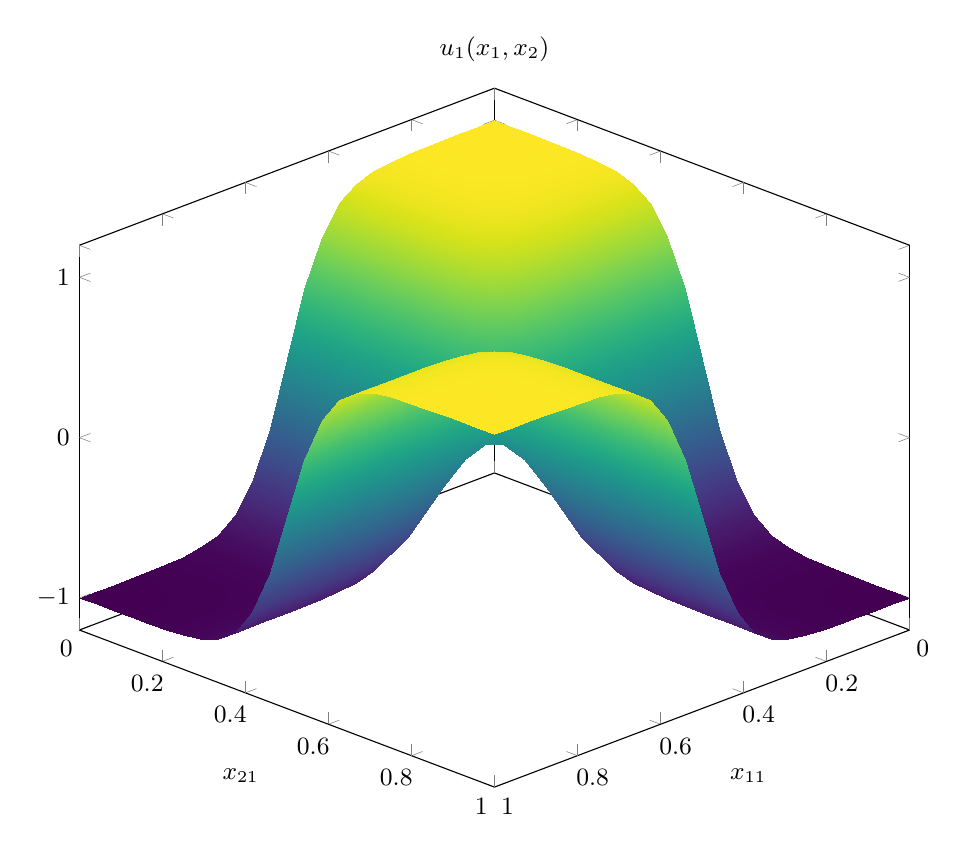
\begin{tikzpicture}
\begin{axis}[
    font=\small,
    domain=0:1,
    y domain=0:1,
    xlabel=$x_{11}$,
    ylabel=$x_{21}$,
    title={$u_1(x_1,x_2)$},
    colormap/viridis,
    view={135}{30},
    mesh/ordering=y varies,
    width=\textwidth,
]
\addplot3[
    surf,
    shader=interp,
]
{
    (
        (exp(10*y) / (exp(10*y) + exp(10*(1 - y))) - exp(10*(1 - y)) / (exp(10*y) + exp(10*(1 - y))))
        *
        (exp(10*x) / (exp(10*x) + exp(10*(1 - x))) - exp(10*(1 - x)) / (exp(10*x) + exp(10*(1 - x))))
    )
};
\end{axis}
\end{tikzpicture}
\end{minipage}


\begin{example}\label{ex.ratliff13.location}
A general-sum 2-player game in $1 \times 1$ variables on the interval
\[
x_i \in [-\pi, \pi] \quad \forall i \in \{1,2\}.
\]
The utility functions are given by
\begin{align*}
u_{1}\left( x_{1}, x_{2} \right) &= \cos\left( x_{11} \right) - \alpha_1 \cos\left( x_{11} - x_{21} \right) \\
u_{2}\left( x_{1}, x_{2} \right) &= \cos\left( x_{21} \right) - \alpha_2 \cos\left(  - x_{11} + x_{21} \right).
\end{align*}
\textcite[Location Game]{ratliff.burden.ea:characterization} studied this game with $\alpha = [1, 1.05]$, in which case the game has two NE: at $(x_1, x_2)$ equal to $(1,-1.1)$, or $(-1,1.1)$.
\end{example}

\begin{example}\label{ex.kroupa21.5}
A 3-player polynomial network game in $1 \times 1 \times 1$ variables on the interval
$$x_{i1} \in [0,1] \quad \forall i \in \{1,2,3\}.$$
The utilities \cite[Example 5]{kroupa.vannucci.ea:separable} are
\begin{align*}
u_{1}\left( x_{1}, x_{2}, x_{3} \right) &=  - x_{21} - 2 x_{31} - 2 x_{11}^{2} + 5 x_{11} x_{21} - 4 x_{11} x_{31} - 2 x_{21}^{2} x_{11} \\
u_{2}\left( x_{1}, x_{2}, x_{3} \right) &= x_{21} - 2 x_{11}^{2} - 5 x_{11} x_{21} - 2 x_{21}^{2} + 5 x_{21} x_{31} + 2 x_{21}^{2} x_{11} - 2 x_{31}^{2} x_{21} \\
u_{3}\left( x_{1}, x_{2}, x_{3} \right) &= 2 x_{31} + 4 x_{11}^{2} + 4 x_{11} x_{31} + 2 x_{21}^{2} - 5 x_{21} x_{31} + 2 x_{31}^{2} x_{21}
\end{align*}
The game has the following $\epsilon$-NE:
\begin{align*}
\mu_1^\star &= 0.291\delta_{-0.056} + 0.191\delta_{-0.066} + 0.518\delta_{-0.06} \\
\mu_2^\star &= 0.232\delta_{0.347} + 0.147\delta_{0.359} + 0.622\delta_{0.352} \\
\mu_3^\star &= 0.281\delta_{-1.0} + 0.719\delta_{1.0}.
\end{align*}
\end{example}

\begin{example}\label{ex.kroupa21.6}
A 4-player game in $4 \times 4 \times 2 \times 2$ variables constrained to the scaled simplexes:
\begin{align*}
x_i &\in \left\{ z \in \mathbb{R}^4 \ \middle|\ z_i \ge 0,\ \sum_{i=1}^m z_i = a_i \right\} \quad \forall i \in \{1,2\},\\
x_i &\in \left\{ z \in \mathbb{R}^2 \ \middle|\ z_i \ge 0,\ \sum_{i=1}^m z_i = 1 \right\} \quad \forall i \in \{3,4\}.
\end{align*}
The utilities are defined by
\begin{align*}
u_1(x_1, x_2, x_3, x_4) &= a_{1} - f_{1}(x_{11}, x_{31}) - f_{2}(x_{12}, x_{32}) - f_{3}(x_{13}, x_{41}) - f_{4}(x_{14}, x_{42}) - o \\
u_2(x_1, x_2, x_3, x_4) &= a_{2} - f_{1}(x_{21}, x_{31}) - f_{2}(x_{22}, x_{32}) - f_{3}(x_{23}, x_{41}) - f_{4}(x_{24}, x_{42}) - o \\
u_3(x_1, x_2, x_3, x_4) &= f_{1}(x_{11}, x_{31}) + f_{2}(x_{12}, x_{32}) + f_{1}(x_{21}, x_{31}) + f_{2}(x_{22}, x_{32}) -  o \\
u_4(x_1, x_2, x_3, x_4) &= f_{3}(x_{13}, x_{41}) + f_{4}(x_{14}, x_{42}) + f_{3}(x_{23}, x_{41}) + f_{4}(x_{24}, x_{42})  -  o
\end{align*}
where $a=[0.5, 0.8]$, $o=0.325$, and $f$ are the \emph{efficiency} functions:
\begin{align*}
f_1(u,v) &= (1-v^2)0.7u^2\\
f_2(u,v) &= (1-v)^2(1.4u - 0.7u^2)\\
f_3(u,v) &= (1-v^2)(1.8u - 0.9u^2)\\
f_4(u,v) &= (1-v)^20.9u^2
\end{align*}
This polynomial security game was studied by \textcite[Example 6]{kroupa.vannucci.ea:separable}.
\end{example}



\begin{example}\label{ex.yasodharan19}
A general-sum 2-player game in $(m+1) \times 1$ variables on the unit hypercubes
\begin{align*}
    x_1 &\in [0,1]^{m+1}\\
    x_2 &\in [0,1].
\end{align*}
The utility functions are given by
\begin{align*}
u_1(x_1, x_2) &= \sum_{\substack{i=0,\dots,m\\j=i+1}} x_{1j} \binom{m}{i} x_{21}^i (1 - x_{21})^{m - i} - \frac{\gamma}{2^m} \sum_{\substack{i=0,\dots,m\\j=i+1}} x_{1j} \binom{m}{i} - 1 \\
u_2(x_1, x_2) &= - (x_{21} - 0.8)^2 + \sum_{\substack{i=0,\dots,m\\j=i+1}} \binom{m}{i} (1 - x_{1j}) x_{21}^i (1 - x_{21})^{m - i}.
\end{align*}
This example is based on the \emph{hypothesis testing game} by \textcite{yasodharan.loiseau:nonzero-sum}.
\end{example}

\iffalse
\begin{example}\label{ex.misc.square.diff}
A two-player zero-sum game in $1 \times 1$ variables on the interval
$$x_{i1} \in [-1,1] \quad \forall i \in \{1,2\}.$$
The utility function is the difference of squares:
\begin{align*}
u_{1}\left( x_{1}, x_{2} \right) =  - x_{11}^{2} + x_{21}^{2}
\end{align*}
The game has the pure equilibrium $x^\star = (0,0)$.
\end{example}

\noindent
\begin{minipage}[c]{0.6\textwidth}
\begin{example}\label{ex.misc.monkey.saddle}
A two-player zero-sum game in $1 \times 1$ variables on the interval
$$x_{i1} \in [-1,1] \quad \forall i \in \{1,2\}.$$
The utility function is the \emph{monkey saddle}
\begin{align*}
u_{1}\left( x_{1}, x_{2} \right) &= x_{11}^{3} - 3 x_{21}^{2} x_{11}
\end{align*}
This game has the following mixed $\epsilon$-NE:
\begin{align*}
\mu_1^\star &\approx \frac{1}{3}\delta_{ (1.0,) } + \frac{2}{3}\delta_{ (-0.5,) }, \\
\mu_2^\star &\approx \frac{1}{4}\delta_{ (-1.0,) } + \frac{3}{4}\delta_{ (0.0,) }.
\end{align*}

\end{example}
\end{minipage}
\hfill
\begin{minipage}[c]{0.35\textwidth}
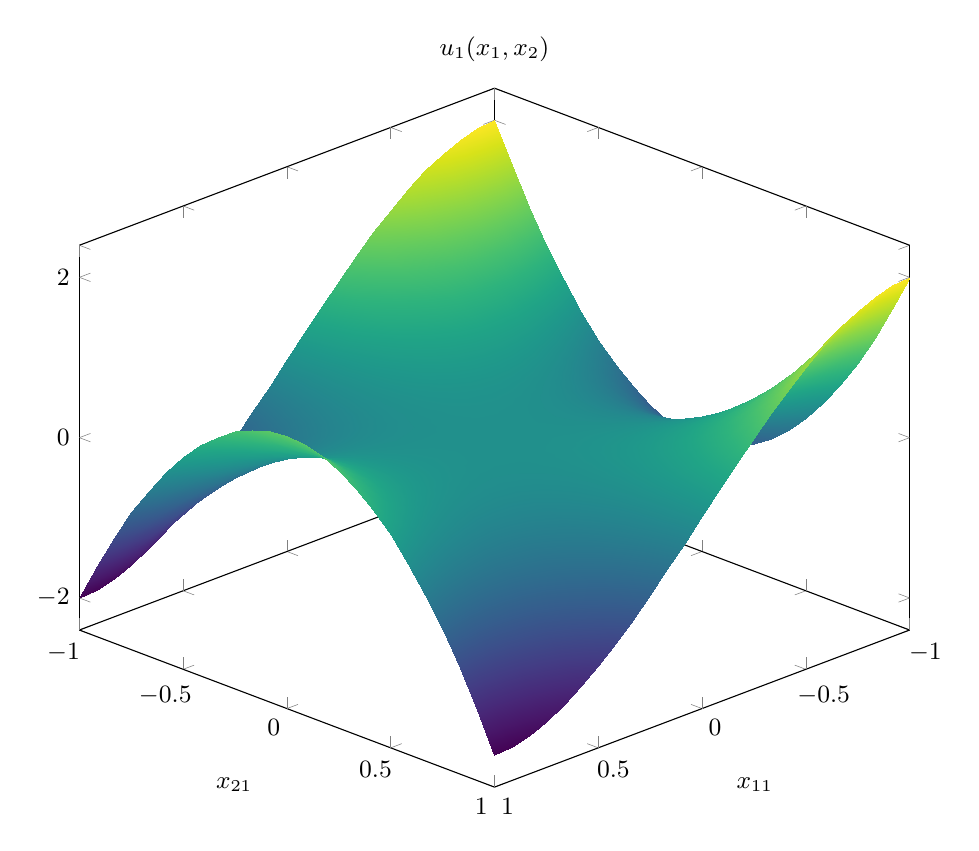
\begin{tikzpicture}
\begin{axis}[
    font=\small,
    domain=-1:1,
    y domain=-1:1,
    xlabel=$x_{11}$,
    ylabel=$x_{21}$,
    title={$u_1(x_1,x_2)$},
    colormap/viridis,
    view={135}{30},
    mesh/ordering=y varies,
    width=\textwidth,
]
\addplot3[
    surf,
    shader=interp,
]
{x^3-3*x*y^2};
\end{axis}
\end{tikzpicture}
\end{minipage}

\begin{example}\label{ex.misc.mul.div}
A general-sum 2-player game in $1 \times 1$ variables on the interval
$$x_{i1} \in [-3,-1] \quad \forall i \in \{1,2\}.$$
The utility functions are given by
\begin{align*}
u_{1}\left( x_{1}, x_{2} \right) &=  - 2 x_{11} x_{21} \\
u_{2}\left( x_{1}, x_{2} \right) &= \frac{2 x_{11}}{x_{21}}.
\end{align*}
The game has a pure Nash equilibrium $x^\star = (-1, -1)$.
\end{example}
\fi

\begin{example}\label{ex.nguyen23.iv}
A 6-player game in $1 \times 1 \times 1 \times 1 \times 1 \times 1$ variables
on the interval
$$x_{i1} \in [x_{\min},x_{\max}] \quad \forall i \in \{1,\dots,6\}.$$
The utility functions are defined by:
$$
u_i(x) = -\eta_ix_{i1}+\beta_i \left(\ln \left(1+a_i\frac{\gamma_i(x)}{1-\Phi_{ii}\gamma_i(x)} \right)-x_{i1}\right) \quad \forall i \in \{1,\dots,6\},
$$
where $\eta_i$, $\beta_i$, and $a_i$ are channel-specific parameters. The parameter $\gamma_i(x)$ represents the \textsc{osnr} \cite{osnr}, defined as
$$
\gamma_i(x) = \frac{x_{i1}}{n_0+\sum_j\Phi_{ij}x_{j1}},
$$
for a given system matrix $\Phi$ and input noise $n_0$. The numerical setting is adopted from an article by \textcite{nguyen.bianchi.ea:nash}. Specifically, $n_0=0.43\times10^{-6}$, $\eta_1=\dots=\eta_6=1$,
\begin{align*}
    \beta & = [0.5, 0.51, 0.52, 0.3, 0.31, 0.32],\\ a & = [0.261, 0.494, 0.107, 0.366, 0.208, 0.305],
\end{align*}
 $x_{\min} = 0.2$, $x_{\max} = 2$, and the matrix
\[
\Phi = \begin{bmatrix}
7.463 & 7.378 & 7.293 & 7.210 & 7.127 & 6.965 \\
7.451 & 7.365 & 7.281 & 7.198 & 7.115 & 6.953 \\
7.438 & 7.353 & 7.269 & 7.186 & 7.103 & 6.942 \\
7.427 & 7.342 & 7.258 & 7.175 & 7.093 & 6.931 \\
7.409 & 7.324 & 7.240 & 7.157 & 7.075 & 6.914 \\
7.387 & 7.303 & 7.219 & 7.136 & 7.055 & 6.894
\end{bmatrix}
\times 10^{-5}.
\]
The game has a Nash equilibrium $x^\star \approx [0.3329, 0.3375, 0.3412, 0.2305, 0.2361, 0.2421]$.
\end{example}

\subsection{Rational Saddle Point Games}

The following examples are the saddle point problems of rational polynomials studied by \textcite{zhou.wang.ea:saddle}, which we interpret here as two-player zero-sum games where each player controls multiple variables.

\begin{example}\label{ex.zhou19.5.3.i}
A two-player zero-sum game in $2 \times 2$ variables on the unit hypercube
\[
x_i \in [0,1]^2 \quad \forall i \in \{1,2\}.
\]
The rational utility function \cite[Example 5.3 (i)]{zhou.wang.ea:saddle} is given by
\[
u_1(x_1, x_2) =
\frac{
- x_{11}^2 - x_{12}^2 + x_{21}^2 + x_{22}^2
}{
x_{11} + x_{22} + 1
}
\]
This game has a pure Nash equilibrium at
\begin{align*}
x_1^\star = (0, 0),\, x_2^\star = (0, 0).
\end{align*}
\end{example}


\begin{example}\label{ex.zhou19.5.3.ii}
A two-player zero-sum game in $3 \times 3$ variables on the unit hypercube
\[
x_i \in [0,1]^3 \quad \forall i \in \{1,2\}.
\]
The rational utility function \cite[Example 5.3 (ii)]{zhou.wang.ea:saddle} is given by
\[
u_1(x_1, x_2) =
\frac{
- \sum_{i=1}^{3} (x_{1i} + x_{2i}) - \sum_{\substack{i=1 \\ i < j}}^{3} \sum_{j=1}^{3} (x_{1i}^2 x_{2j}^2 - x_{2i}^2 x_{1j}^2)
}{
x_{11}^2 + x_{22}^2 + x_{13} x_{23} + 1
}
\]
This game has no pure Nash equilibria.
\end{example}





\section{Optimization Test Functions}
Following the idea of \textcite{adam.horčík.ea:double}, who used a constrained-optimization example as the utility function of a two-player zero-sum game in \cref{ex.adam21.townsend}, we constructed games based on the dataset of optimization test functions by \textcite{surjanovic13}. Specifically, we selected one example from each shape category: many local minima, bowl-shaped, plate-shaped, valley-shaped, steep ridges, and other.

\strut

\noindent
\begin{minipage}[c]{0.6\textwidth}
\begin{game}\label{ex.adam21.townsend}
A two-player zero-sum game in $1 \times 1$ variables constrained to the intervals
\begin{align*}
x_{11} &\in [-2.25,2.5]\\
x_{21} &\in [-2.5,1.75]
\end{align*}
with the utility given by the \emph{Townsend} function
\begin{align*}
u_1(x_{1}, x_{2}) = x_{11} \sin\left( 3 x_{11} + x_{21} \right) + \cos^{2}\left( \left(x_{11}-0.1 \right) x_{21} \right)
\end{align*}
This game was studied by \textcite[Townsend]{adam.horčík.ea:double}.
\end{game}
\strut
\end{minipage}
\hfill
\begin{minipage}[c]{0.35\textwidth}
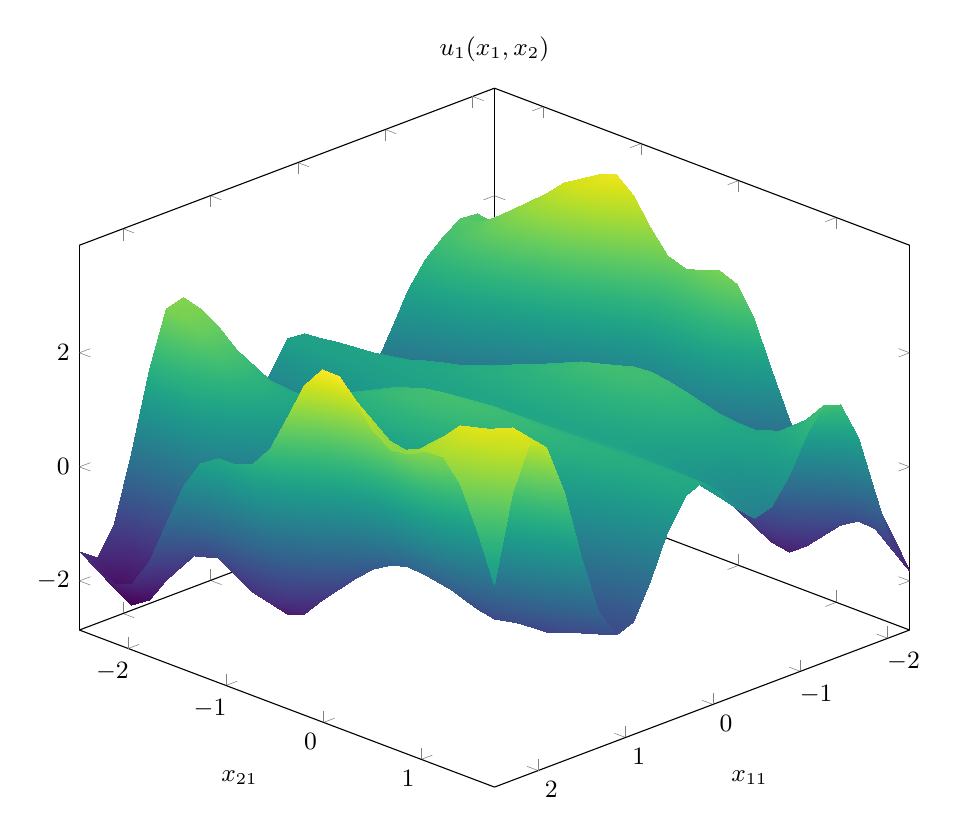
\begin{tikzpicture}
\begin{axis}[
    font=\small,
    domain=-2.25:2.5,
    y domain=-2.5:1.75,
    xlabel=$x_{11}$,
    ylabel=$x_{21}$,
    title={$u_1(x_1,x_2)$},
    colormap/viridis,
    view={135}{30},
    mesh/ordering=y varies,
    width=\textwidth,
]
\addplot3[
    surf,
    shader=interp,
]
{cos(deg((x - 0.1) * y))^2 + x * sin(deg(3 * x + y))};
\end{axis}
\end{tikzpicture}
\end{minipage}



\noindent
\begin{minipage}[c]{0.6\textwidth}
\begin{game}\label{ex.surjanovic.ackley}
A two-player zero-sum game in $1 \times 1$ variables on the interval
\begin{align*}
    x_i &\in [-32.768,32.768] \quad \forall i \in \{1,2\}
\end{align*}
with the utility function \cite[Ackley]{surjanovic13}
\begin{align*}
u_{1}(x_{1}, x_{2}) &=-a e^{-b \sqrt{\frac{1}{2}\sum_{i=1}^2 x_i^2}} - e^{\frac{1}{2}\sum_{i=1}^2\cos(cx_i)} + a + e
\end{align*}
where $a=20$, $b=0.2$, and $c=2\pi$.
\end{game}
\strut
\end{minipage}
\hfill
\begin{minipage}[c]{0.35\textwidth}
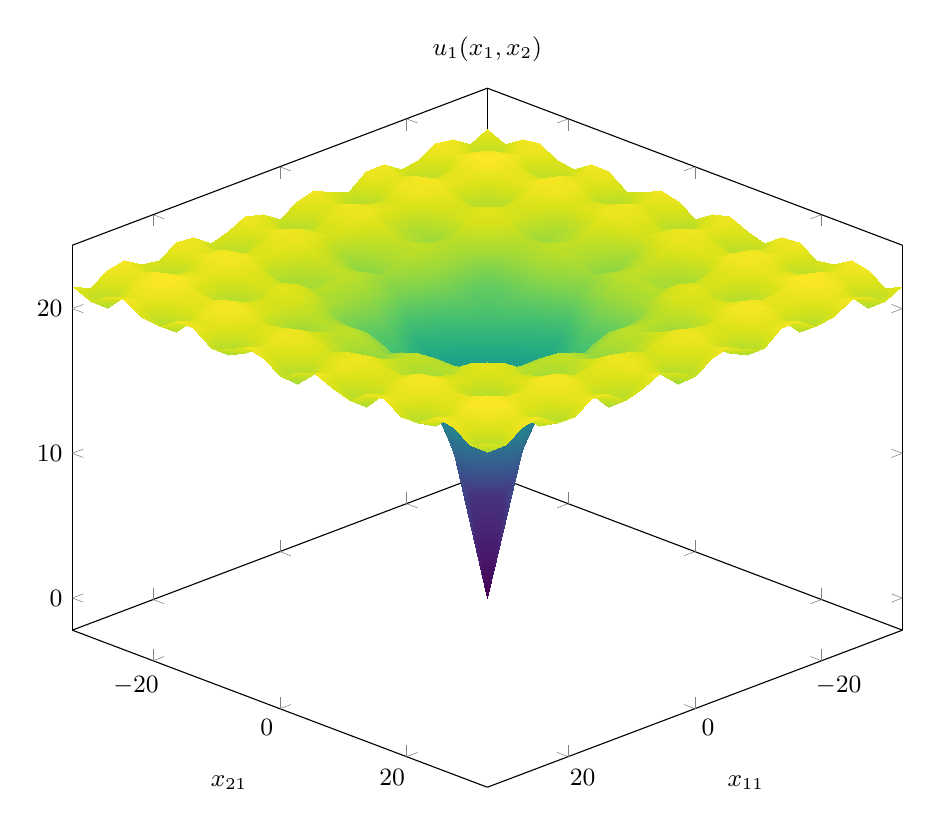
\begin{tikzpicture}
\begin{axis}[
    font=\small,
    domain=-32.768:32.768,
    y domain=-32.768:32.768,
    xlabel=$x_{11}$,
    ylabel=$x_{21}$,
    title={$u_1(x_1,x_2)$},
    colormap/viridis,
    view={135}{30},
    point meta min=5,
    width=\textwidth,
]
\addplot3[
    surf,
    shader=interp,
]
{-20*exp(-0.2 * sqrt((x^2 + y^2)/(2))) - exp((cos(deg(2*pi*x)) + cos(deg(2*pi*y)))/(2)) + 20 + exp(1)};
\end{axis}
\end{tikzpicture}
\end{minipage}




\noindent
\begin{minipage}[c]{0.6\textwidth}
\begin{game}\label{ex.surjanovic.boha1}
A two-player zero-sum game in $1 \times 1$ variables on the interval
\begin{align*}
    x_i &\in [-100,100] \quad \forall i \in \{1,2\}
\end{align*}
with the utility function \cite[Bohachevsky 1]{surjanovic13}
\begin{align*}
u_{1}( x_{1}, x_{2}) &= - 0.3\cos(3\pi x_1) - 0.4\cos(4 \pi x_2) \\ &+  x_1^2 + 2 x_2^2 + 0.7
\end{align*}
\end{game}
\strut
\end{minipage}
\hfill
\begin{minipage}[c]{0.35\textwidth}
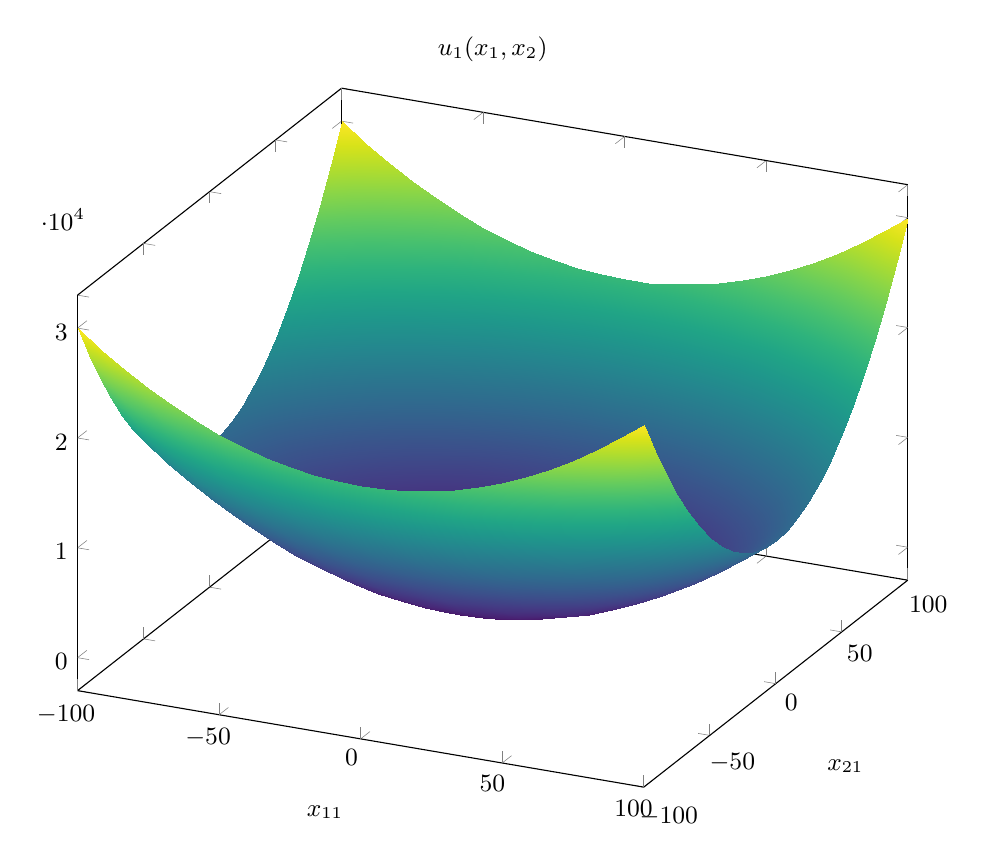
\begin{tikzpicture}
\begin{axis}[
    font=\small,
    domain=-100:100,
    y domain=-100:100,
    xlabel=$x_{11}$,
    ylabel=$x_{21}$,
    title={$u_1(x_1,x_2)$},
    colormap/viridis,
    mesh/ordering=y varies,
    width=\textwidth,
]
\addplot3[
    surf,
    shader=interp,
]
{x^2 + 2 * y^2 - 0.3 * cos(deg(3 * pi * x)) - 0.4 * cos(deg(4 * pi * y)) + 0.7};
\end{axis}
\end{tikzpicture}
\end{minipage}




\noindent
\begin{minipage}[c]{0.6\textwidth}
\begin{game}\label{ex.surjanovic.branin}
A two-player zero-sum game in $1 \times 1$ variables on the intervals
\begin{align*}
    x_1 &\in [-5,10] \\
    x_2 &\in [0,15]
\end{align*}
with the utility function \cite[Branin]{surjanovic13}
\begin{align*}
u_{1}( x_{1}, x_{2} ) &= a (x_2 - b  x_1^2 + c  x_1 - r)^2 \\ &+  s (1 - t) \cos(x_1) + s
\end{align*}
where $a=1$, $b=\frac{5.1}{4 \pi^2}$, $c=\frac{5}{\pi}$, $r=6$, $s=10$, $t=\frac{1}{8\pi}$.

\end{game}
\strut
\end{minipage}
\hfill
\begin{minipage}[c]{0.35\textwidth}
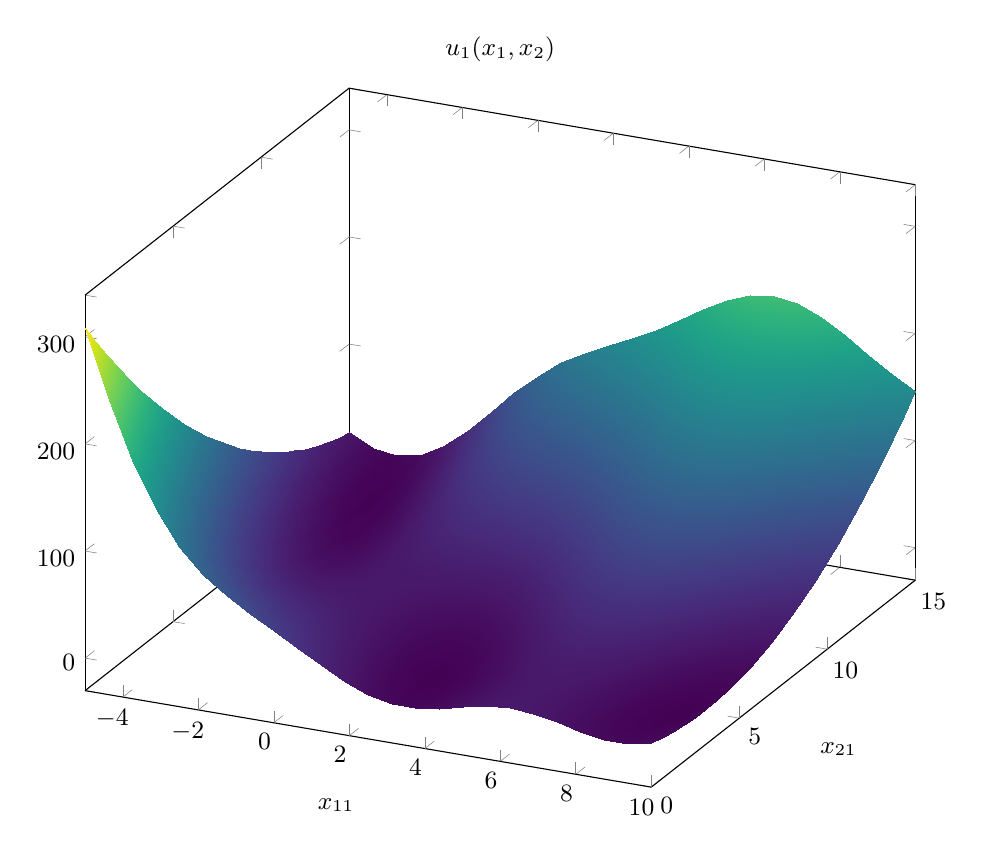
\begin{tikzpicture}
\begin{axis}[
    font=\small,
    domain=-5:10,
    y domain=0:15,
    xlabel=$x_{11}$,
    ylabel=$x_{21}$,
    title={$u_1(x_1,x_2)$},
    colormap/viridis,
    width=\textwidth,
]
\addplot3[
    surf,
    shader=interp,
]
{(y - 5.1 / (4 * pi^2) * x^2 + (5/pi) * x - 6)^2 +  10 * (1 - 1 / (8 * pi)) * cos(deg(x)) + 10};
\end{axis}
\end{tikzpicture}
\end{minipage}




\noindent
\begin{minipage}[c]{0.6\textwidth}
\begin{game}\label{ex.surjanovic.mccorm}
A two-player zero-sum game in $1 \times 1$ variables on the intervals
\begin{align*}
    x_1 &\in [-1.5,4] \\
    x_2 &\in [-3,4]
\end{align*}
with the utility function \cite[McCormick]{surjanovic13}
\begin{align*}
u_{1}{\left( x_{1}, x_{2} \right)} &= \sin(x_1 + x_2) + (x_1 - x_2)^2 - \frac{3x_1 + 5x_2 + 2}{2}
\end{align*}

\end{game}
\strut
\end{minipage}
\hfill
\begin{minipage}[c]{0.35\textwidth}
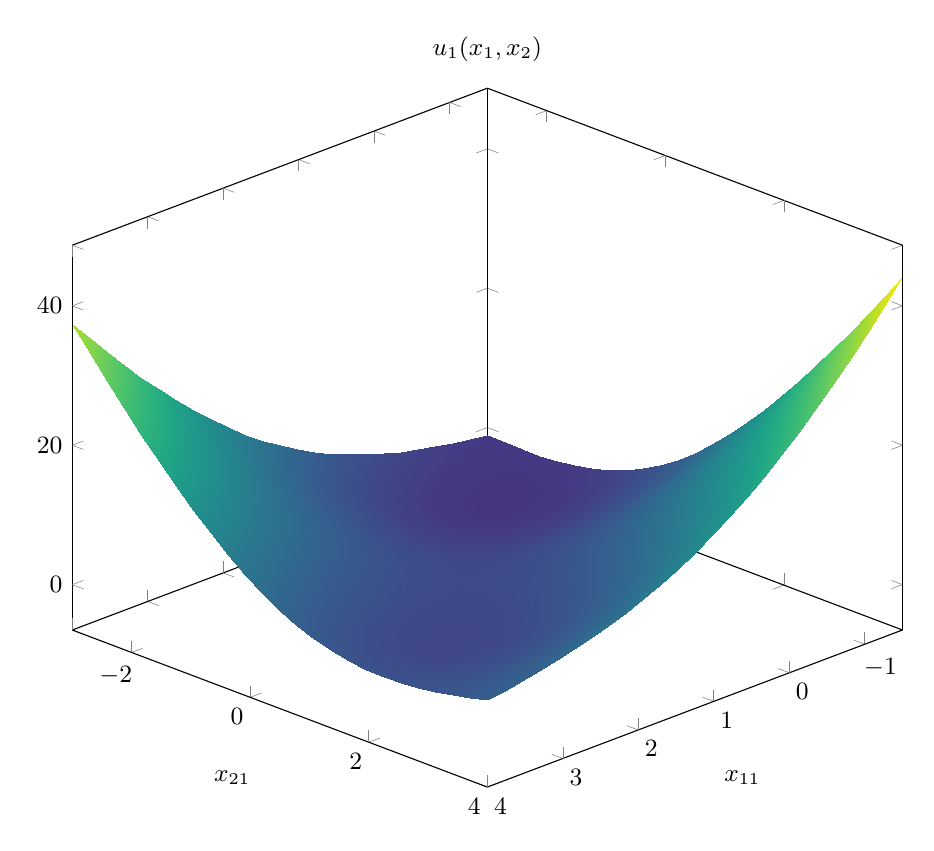
\begin{tikzpicture}
\begin{axis}[
    font=\small,
    domain=-1.5:4,
    y domain=-3:4,
    xlabel=$x_{11}$,
    ylabel=$x_{21}$,
    title={$u_1(x_1,x_2)$},
    colormap/viridis,
    view={135}{30},
    mesh/ordering=y varies,
    point meta min=-10,
    width=\textwidth,
]
\addplot3[
    surf,
    shader=interp,
]
{sin(deg(x + y)) + (x - y)^2 - 1.5*x + 2.5*y + 1};
\end{axis}
\end{tikzpicture}
\end{minipage}



\noindent
\begin{minipage}[c]{0.6\textwidth}
\begin{game}\label{ex.surjanovic.michal}
A two-player zero-sum game in $1 \times 1$ variables on the interval
\begin{align*}
    x_i &\in [0,\pi] \quad \forall i \in \{1,2\}
\end{align*}
with the utility function \cite[Michalewicz]{surjanovic13}
\begin{align*}
u_{1}{\left( x_{1}, x_{2} \right)} &= -\sum_{i=1}^2 \sin(x_i) \sin^{2m}{\left(\frac{i x_i^2}{\pi}\right)}
\end{align*}
where $m=20$.
\end{game}
\strut
\end{minipage}
\hfill
\begin{minipage}[c]{0.35\textwidth}
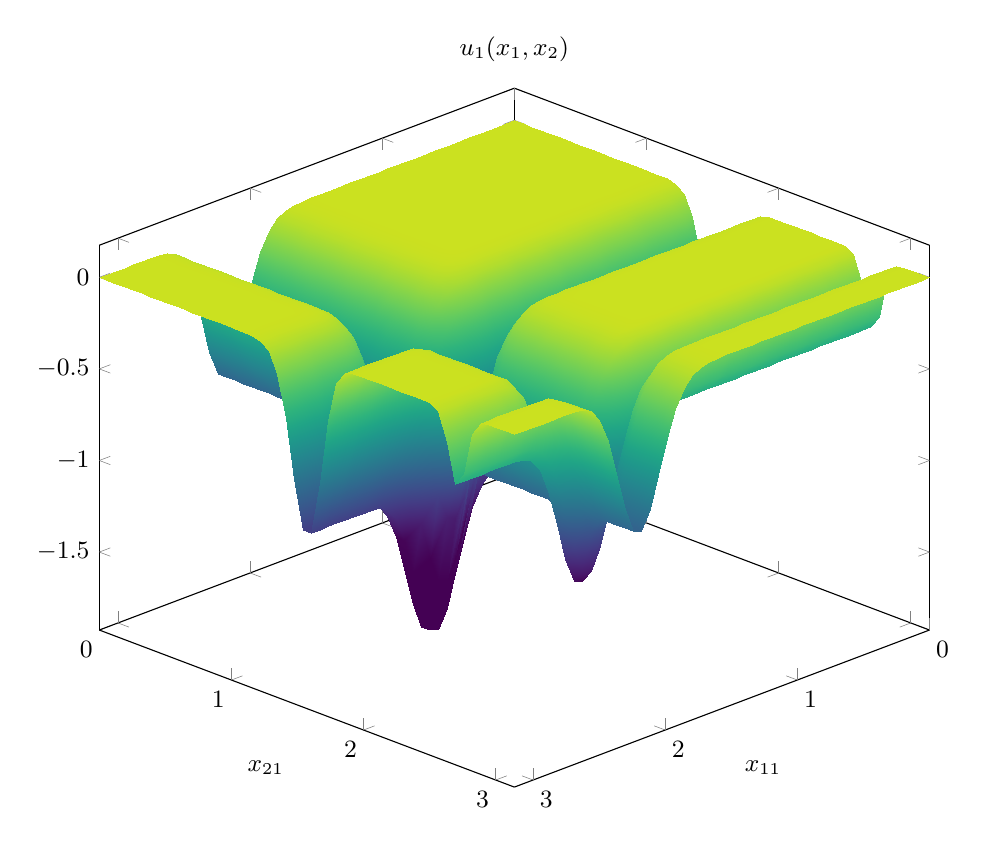
\begin{tikzpicture}
\begin{axis}[
    font=\small,
    domain=0:pi,
    y domain=0:pi,
    samples=50,
    xlabel=$x_{11}$,
    ylabel=$x_{21}$,
    title={$u_1(x_1,x_2)$},
    colormap/viridis,
    view={135}{30},
    mesh/ordering=y varies,
    point meta max=0.1,
    point meta min=-1.2,
    width=\textwidth,
]
\addplot3[
    surf,
    shader=interp,
]
{- sin(deg(x)) * sin(deg(x^2/pi))^20 - sin(deg(y)) * sin(deg(2*y^2/pi))^20};
\end{axis}
\end{tikzpicture}
\end{minipage}



\noindent
\begin{minipage}[c]{0.6\textwidth}
\begin{game}\label{ex.surjanovic.rosen}
A two-player zero-sum game in $1 \times 1$ variables on the interval
\begin{align*}
    x_i &\in [-5,10] \quad \forall i \in \{1,2\}
\end{align*}
with the utility function \cite[Rosenbrock]{surjanovic13}
\begin{align*}
u_{1}{\left( x_{1}, x_{2} \right)} &= 100 (y - x^2)^2 + (x - 1)^2
\end{align*}
\end{game}
\strut
\end{minipage}
\hfill
\begin{minipage}[c]{0.35\textwidth}
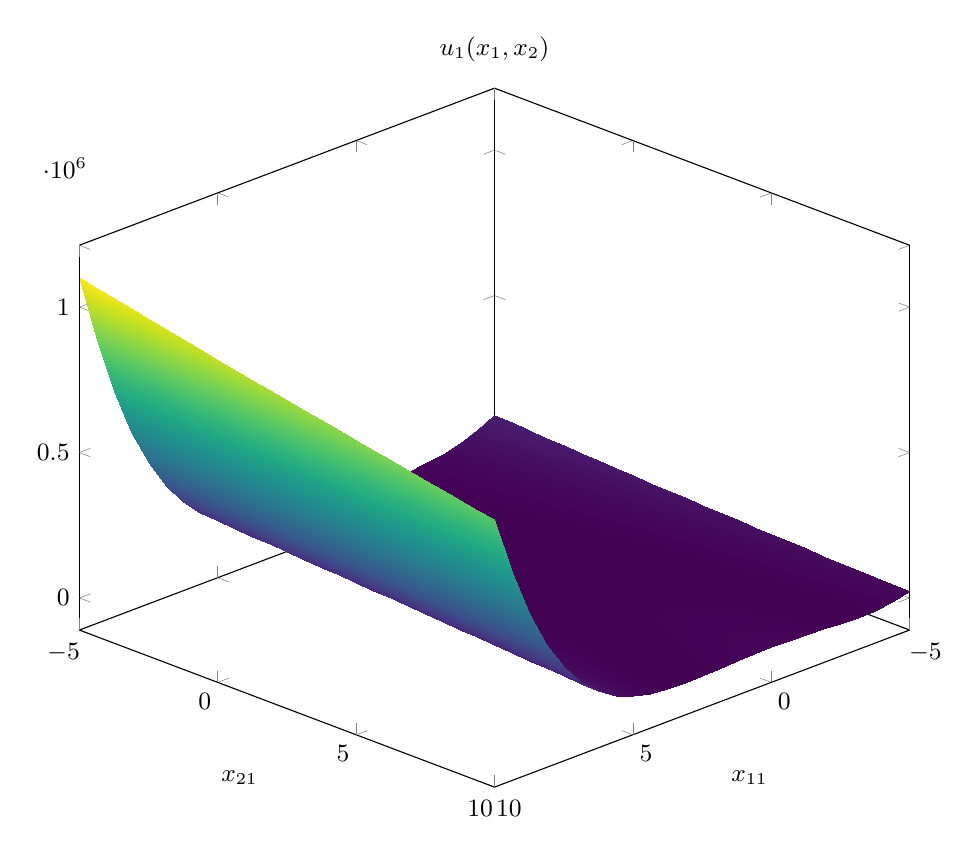
\begin{tikzpicture}
\begin{axis}[
    font=\small,
    domain=-5:10,
    y domain=-5:10,
    xlabel=$x_{11}$,
    ylabel=$x_{21}$,
    title={$u_1(x_1,x_2)$},
    colormap/viridis,
    view={135}{30},
    mesh/ordering=y varies,
    width=\textwidth,
]
\addplot3[
    surf,
    shader=interp,
]
{100*(y - x^2)^2 + (x - 1)^2 };
\end{axis}
\end{tikzpicture}
\end{minipage}

\section{Non-continuous Games with Known Equilibria}


For completeness, we finish with a small number of games that either contain discontinuities or have non-compact strategy sets. Neither equilibria nor best responses necessarily exist in such games; for this reason, we include only examples with known solutions.

\begin{example}
A two-player zero-sum game in $m \times m$ variables on the simplex
\[
x_i \in \Delta^{m-1} = \left\{ z \in \mathbb{R}^m \ \middle|\ z_j \ge 0,\ \sum_{j=1}^m z_j = 1 \right\} \quad \forall i \in \{1,2\}
\]
The utility is defined by the discontinuous function
\[
u_1(x_1, x_2) = \sum_{i=1}^m \operatorname{sign}\left( x_{1j} - x_{2j} \right)
\]
This is an infinite version of the classical \emph{Colonel Blotto} game \cite{Laslier.colonel,Kvasov.colonel,gross.wagner.colonel,Golman2009}, in which all isolated fronts have equal value. Pure strategies exist only for $m \in \{1,2\}$, in which case every strategy is a tie; or for $m=3$, when players should allocate $\frac{1}{3}$ to every front. Otherwise, \textcite{roberson.colonel} proved that players must play a strategy with marginals $\mu^\star_{ij} = \mathcal{U}\left[0,\frac{2}{m}\right]$ for every front $j$.
\end{example}


\subsection{Unbounded Polynomial Saddle Point Games}
The following polynomial games are played over unbounded strategy sets.

\begin{game}
A zero-sum 2-player game in $4 \times 4$ variables on the nonnegative orthant
\[
x_i \in \mathbb{R}^4_+ \quad \forall i \in \{1,2\}
\]
with the utility function \cite[Example~6.7]{nie.yang.ea:saddle}
\begin{align*}
u_1(x_1, x_2) = &-x_{21}(x_{12} + x_{13} + x_{14} - 1)^2 - x_{22}(x_{11} + x_{13} + x_{14} - 2)^2 \\
    &- x_{23}(x_{11} + x_{12} + x_{14} - 3)^2 + x_{24}(x_{11} + x_{12} + x_{13} - 4)^2 \\
    &+ x_{11}(x_{22} + x_{23} + x_{24} - 1)^2 + x_{12}(x_{21} + x_{23} + x_{24} - 2)^2 \\
    &- x_{13}(x_{21} + x_{22} + x_{24} - 3)^2 + x_{14}(x_{21} + x_{22} + x_{23} - 4)^2
\end{align*}
The game has a pure Nash equilibrium:
\begin{align*}
x_1^\star \approx (1.5075, 0.5337, 0.0000, 0.5018), \\
x_2^\star \approx (2.4143, 1.1463, 0.0000, 0.0000).
\end{align*}
\end{game}

\begin{game}
A zero-sum 2-player game in $3 \times 3$ variables with no constraints
\[
x_i \in \mathbb{R}^3 \quad \forall i \in \{1,2\}.
\]
The utility function \cite[Example~6.8]{nie.yang.ea:saddle} is
\[
u_1(x_1, x_2) = -\sum_{i=1}^{3} (x_{1i}^4 - x_{2i}^4 + x_{1i} + x_{2i}) - \sum_{i=1}^{3} \sum_{\substack{j=1 \\ i \ne j}}^{3} x_{1i}^3 x_{2j}^3
\]
The game has a pure Nash equilibrium:
\begin{align*}
x_1^\star \approx −(0.6981, 0.6981, 0.6981), \\
x_2^\star \approx (0.4979, 0.4979, 0.4979).
\end{align*}
\end{game}

\begin{game}
A zero-sum 2-player game in $3 \times 3$ variables subject to the constraints
\[
x_i \in \left\{z \in \mathbb{R}^3 \,\middle|\, z_1 \geq 0, z_1z_2 \geq 1, z_2z_3 \geq 1 \right\} \quad \forall i \in \{1,2\}
\]
which define a non-compact set. The utility function \cite[Example~6.9]{nie.yang.ea:saddle} is
\[
u_1(x_1, x_2) = -x_{11}^3x_{21} - x_{12}^3x_{22} - x_{13}^3x_{23} + 3x_{11}x_{12}x_{13} + x_{21}^2 + 2x_{22}^2 + 3x_{23}^2
\]
The game has a pure Nash equilibrium:
\begin{align*}
x_1^\star \approx (1.2599, 1.2181, 1.3032), \\
x_2^\star \approx (1.0000, 1.1067, 0.9036).
\end{align*}
\end{game}

\subsection{Discontinuous Rational Saddle Point Games}


The following games were created from the saddle point problems of rational polynomials studied by \textcite{zhou.wang.ea:saddle}. The utility functions are not continuous on the whole strategy set as the divisor often vanishes on the boundary.

\begin{game}\label{ex.zhou19.5.1}

A two-player zero-sum game in $3 \times 3$ variables on the simplex
\[
x_i \in \Delta^{2} \quad \forall i \in \{1,2\}.
\]
The rational utility function \cite[Example~5.1]{zhou.wang.ea:saddle} is given by
\[
u_1(x_1, x_2) =
\frac{
- \sum_{i=1}^{3} \sum_{j=1}^{3} x_{1i}^2 x_{2j}^2 + \sum_{i=1}^{3} \sum_{\substack{j=1 \\ i \ne j}}^{3} (x_{1i} x_{1j} + x_{2i} x_{2j})
}{
x_{11} + x_{12} + x_{22} + x_{23}
}
\]
This game has two pure Nash equilibria:
\begin{align*}
\text{NE}_1: &x_1^\star \approx (0.3165, 0.3165, 0.3670),\,x_2^\star = (0, 1, 0),\\
\text{NE}_2: &x_1^\star \approx (0.3165, 0.3165, 0.3670),\,x_2^\star = (0, 0, 1).
\end{align*}
\end{game}

\begin{game}\label{ex.zhou19.5.2.ii}
A two-player zero-sum game in $3 \times 3$ variables on the hypercube
\[
x_i \in [-1,1]^3 \quad \forall i \in \{1,2\}.
\]
The rational utility function \cite[Example~5.2 (ii)]{zhou.wang.ea:saddle} is given by
\[
u_1(x_1, x_2) =
\frac{
- \sum_{i=1}^{3} x_{1i}^2 + \sum_{i=1}^{3} x_{2i}^2
}{
\sum_{i=1}^{3} x_{2i}^2 - \sum_{i=1}^{3} x_{1i}^2 + 3
}
\]
This game has a pure Nash equilibrium at
\begin{align*}
x_1^\star = (0, 0, 0),\, x_2^\star = (0, 0, 0).
\end{align*}
\end{game}

\begin{game}\label{ex.zhou19.5.4.i}
A zero-sum 2-player game in $3 \times 3$ variables on the nonnegative orthant
\[
x_i \in \mathbb{R}^3_+ \quad \forall i \in \{1,2\}
\]
with the utility function \cite[Example~5.4 (i)]{zhou.wang.ea:saddle}
\[
u_1(x_1, x_2) =
\frac{
- x_{11}^4 - x_{12}^4 - x_{13}^4 + x_{21}^4 + x_{22}^4 + x_{23}^4
}{
x_{11} + x_{21} + 1
}
\]
The game has a pure Nash equilibrium:
\begin{align*}
x_1^\star \approx (0.0015, 0.0015, 0.0015), \\
x_2^\star \approx (0.0015, 0.0015, 0.0015).
\end{align*}
\end{game}


\begin{game}\label{ex.zhou19.5.5.i}

A two-player zero-sum game in $2 \times 2$ variables on the ball
\[
x_i \in \left\{ z \in \mathbb{R}^2 \,\middle|\, \norm{z} \leq 1  \right\} \quad \forall i \in \{1,2\}
\]
The rational utility function \cite[Example~5.5 (i)]{zhou.wang.ea:saddle} is
\[
u_1(x_1, x_2) =
\frac{
- x_{11}^2 - x_{12}^2 + 3 x_{11} x_{12} + x_{21}^2 + x_{22}^2 - x_{21} x_{22}
}{
x_{11} x_{21} + 1
}
\]
This game has no pure Nash equilibria.
\end{game}

\begin{game}\label{ex.zhou19.5.5.ii}

A two-player zero-sum game in $3 \times 3$ variables on the ball
\[
x_i \in \left\{ z \in \mathbb{R}^3 \,\middle|\, \norm{z} \leq 1  \right\} \quad \forall i \in \{1,2\}
\]
The rational utility function \cite[Example~5.5 (ii)]{zhou.wang.ea:saddle} is
\[
u_1(x_1, x_2) =
\frac{
- x_{11}^2 x_{21} - 2 x_{12}^2 x_{22} - 3 x_{13}^2 x_{23} + x_{11} + x_{12} + x_{13}
}{
x_{11} x_{21} + 1
}
\]
This game has a pure Nash equilibrium at
\begin{align*}
x_1^\star \approx (0.4730, 0.4476, 0.3416),\, x_2^\star \approx (0.6708, 0.5585, 0.4879).
\end{align*}
\end{game}

\begin{game}\label{ex.zhou19.5.6.i}

A two-player zero-sum game in $3 \times 3$ variables on the sphere
\[
x_i \in \left\{ z \in \mathbb{R}^3 \,\middle|\, \norm{z} = 1  \right\} \quad \forall i \in \{1,2\}
\]
The rational utility function \cite[Example~5.6 (i)]{zhou.wang.ea:saddle} is
\[
u_1(x_1, x_2) =
\frac{
- \sum_{i=1}^{3} (x_{1i}^3 + x_{2i}^3) - 2 (x_{11} x_{12} x_{21} x_{22} + x_{11} x_{13} x_{21} x_{23} + x_{12} x_{13} x_{22} x_{23})
}{
x_{11} - x_{21} + 1
}
\]
The game has no pure NE.
\end{game}

\begin{game}\label{ex.zhou19.5.6.ii}

A two-player zero-sum game in $3 \times 3$ variables on the sphere
\[
x_i \in \left\{ z \in \mathbb{R}^3 \,\middle|\, \norm{z} = 1  \right\} \quad \forall i \in \{1,2\}
\]
The rational utility function \cite[Example~5.6 (ii)]{zhou.wang.ea:saddle} is
\[
u_1(x_1, x_2) =
\frac{
- \sum_{i=1}^{3} (x_{1i}^2 + x_{2i}^2 - x_{1i} - x_{2i})
}{
x_{13} + x_{22} + 2
}
\]
This game has a pure Nash equilibrium at
\begin{align*}
x_1^\star \approx (0.4082, 0.4082, 0.8165),\, x_2^\star \approx (−0.4082, −0.8165, −0.4082).
\end{align*}
\end{game}

\begin{game}\label{ex.zhou19.5.7.i}

A two-player zero-sum game in $3 \times 2$ variables on the intersection of the nonnegative orthant and the n-sphere
\begin{align*}
x_1 &\in \left\{ z \in \mathbb{R}^3_+ \,\middle|\, \norm{z} = 1  \right\} \\
x_2 &\in \left\{ z \in \mathbb{R}^2_+ \,\middle|\, \norm{z} = 1  \right\}
\end{align*}
The rational utility function is
\[
u_1(x_1, x_2) =
\frac{
- \sum_{i=1}^{3} (x_{1i}^2 - x_{1i}) - \sum_{i=1}^{2} (x_{2i} - x_{2i}^2)
}{
x_{11}^2 - x_{21}^2 + 1
}
\]
The utility has a discontinuity at the boundary of $x_1$ when $x_{21} = 1$. \textcite[Example~5.7 (i)]{zhou.wang.ea:saddle} report that this game has no saddle point, although we found the following pure $\epsilon$-NE (with $\epsilon < 10^{-8}$):
\begin{align*}
x_1^\star \approx (0.4351314094, 0.6366555805, 0.6366555805),\, x_2^\star \approx (0.5255286571, 0.8507758992).
\end{align*}
We also show this game reprojected in polar coordinates in \cref{ex.zhou19.5.7.i.polar}, where we recover the same solution.
\end{game}

\begin{game}\label{ex.zhou19.5.7.i.polar}
A two-player zero-sum game in $3 \times 2$ variables on the intersection of the nonnegative orthant and the n-sphere in polar coordinates
\begin{align*}
x_1 &\in \left[0,\frac{\pi}{2} \right]^2 \\
x_1 &\in \left[0,\frac{\pi}{2} \right]
\end{align*}
The utility function is
\[
u_1(x_1, x_2) = \upsilon\left(\bigl[\sin(x_{11}) \cos(x_{12}), \sin(x_{11}) \sin(x_{12}), \cos(x_{11})\bigr], \bigl[\cos(x_{21}), \sin(x_{21}) \bigr] \right)
\]
where
\[
\upsilon(z_1, z_2) = \frac{
- \sum_{i=1}^{3} (z_{1i}^2 - z_{1i}) - \sum_{i=1}^{2} (z_{2i} - z_{2i}^2)
}{
z_{11}^2 - z_{21}^2 + 1
}
\]
This example is the polar coordinate reformulation of the example by \textcite[Example~5.7 (i)]{zhou.wang.ea:saddle}. Despite containing a discontinuity at the boundary of $x_1$ when $x_{21}=0$ the game has the pure $\epsilon$-NE shown in \cref{fig:ex.polar.br}:
\begin{align*}
x_1^\star &\approx (0.8813, 0.9716),\\
x_2^\star &\approx 1.0175.
\end{align*}
\end{game}


\begin{figure}
\centering
\begin{minipage}{0.4\textwidth}
\centering
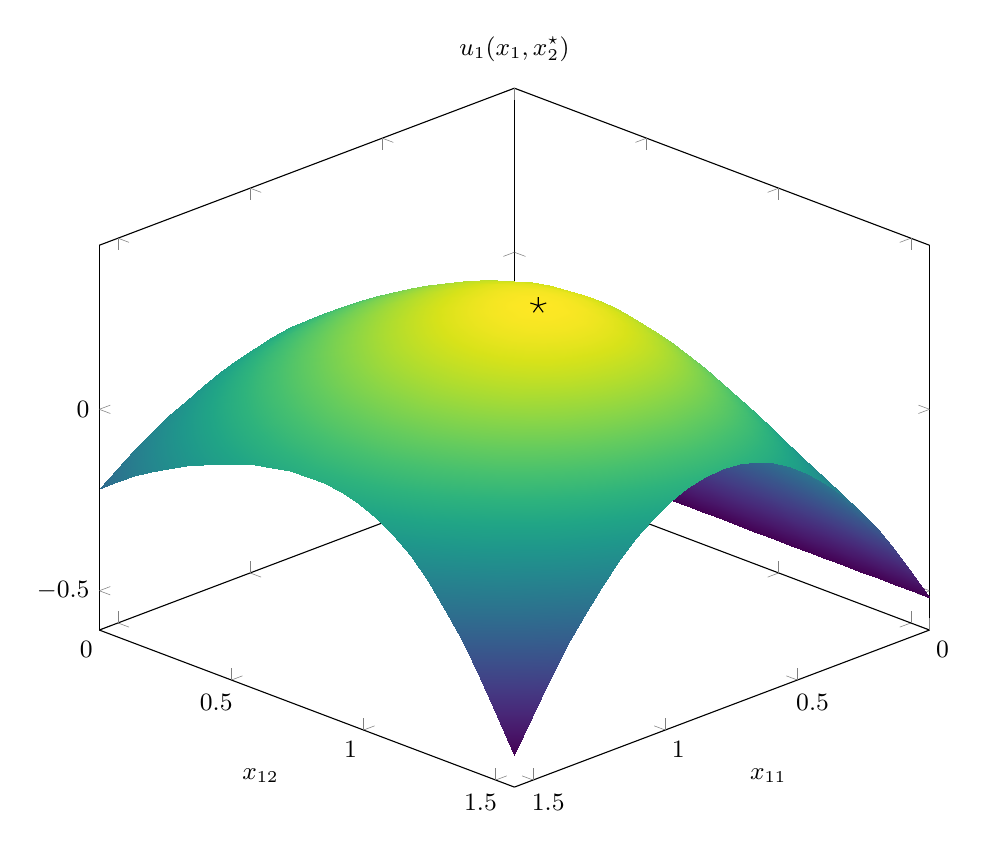
\begin{tikzpicture}
\begin{axis}[
    font=\small,
    domain=0:1.5707963267948966,
    y domain=0:1.5707963267948966,
    xlabel=$x_{11}$,
    ylabel=$x_{12}$,
    title={$u_1(x_1,x_2^\star)$},
    colormap/viridis,
    view={135}{30},
    mesh/ordering=y varies,
    width=\textwidth,
]
\addplot3[
    surf,
    shader=interp,
]
{-((0.376306020901492 - cos(deg(x)) - sin(deg(x))*sin(deg(y)) - sin(deg(x))*cos(deg(y)) + cos(deg(x))^2 + (sin(deg(x))^2)*(sin(deg(y))^2) + (sin(deg(x))^2)*(cos(deg(y))^2)) / (0.7238156036862534 + (sin(deg(x))^2)*(cos(deg(y))^2)))};
\addplot3[
    only marks,
    mark=star,
    color=black,
    mark size=3,
]
coordinates {(0.8812945920343842, 0.9716157415160604, 0.36372376459410616)};
\end{axis}
\end{tikzpicture}
\end{minipage}%
\hspace{1em}
\begin{minipage}{0.4\textwidth}
\centering
\begin{tikzpicture}
\begin{axis}[
    font=\small,
    domain=0:1.5707963267948966,
    xlabel=$x_{21}$,
    title={$u_2(x_1^\star,x_2)$},
    width=0.9\textwidth,
    colormap/viridis,
]
\addplot[
    thick,
]
{(-0.7084434199966159 + sin(deg(x)) + cos(deg(x)) - (sin(deg(x))^2) - (cos(deg(x))^2)) /
 (1.1893427638066412 - (cos(deg(x))^2))};
\addplot[
    only marks,
    mark=star,
    color=black,
    mark size=3,
]
coordinates {(1.0174554472964583, -0.36372376459410616)};
\end{axis}
\end{tikzpicture}
\end{minipage}
\caption{The best-response curves of both players at the $\epsilon$-NE of \cref{ex.zhou19.5.7.i.polar}.}
\label{fig:ex.polar.br}
\end{figure}


\begin{game}\label{ex.zhou19.5.7.ii}
A two-player zero-sum game in $3 \times 3$ variables on the intersection of the nonnegative orthant and the sphere
\[
x_i \in \left\{ z \in \mathbb{R}^3_+ \,\middle|\, \norm{z} = 1  \right\} \quad \forall i \in \{1,2\}
\]
with the utility function \cite[Example~5.7 (ii)]{zhou.wang.ea:saddle}
\[
u_1(x_1, x_2) =
\frac{
- \sum_{i=1}^{3} (x_{1i} - 1)^2 - \sum_{i=1}^{3} (x_{2i} - 1)^2
}{
x_{11}^2 - x_{21}^2 + 1
}
\]
The game has the pure NE
\begin{align*}
x_1^\star \approx (0.9519, 0.2167, 0.2167),\, x_2^\star \approx (1, 0, 0).
\end{align*}
\end{game}

\begin{game}\label{ex.zhou19.5.8.i}
A general-sum 2-player game in $3 \times 3$ variables with no constraints
\[
x_i \in \mathbb{R}^3 \quad \forall i \in \{1,2\}.
\]
with the utility function \cite[Example~5.8 (i)]{zhou.wang.ea:saddle}
\[
u_1(x_1, x_2) =
\frac{
- x_{11}^2 - x_{12}^2 - x_{13}^2 - x_{21}^2 - x_{22}^2 + x_{11} + x_{12}
}{
x_{11}^2 + x_{23}^2 + 1
}
\]
The game has a pure Nash equilibrium:
\begin{align*}
x_1^\star \approx (0.3508, 0.5000, 0.0000), \\
x_2^\star \approx (0.0000, 0.0000, 0.0000).
\end{align*}
\end{game}

\begin{game}\label{ex.zhou19.5.9.i}
A zero-sum 2-player game in $3 \times 3$ variables subject to the constraints
\[
x_i \in \left\{z \in \mathbb{R}^3 \,\middle|\, z_1 \geq 0, z_1z_2 \geq 1, z_2z_3 \geq 1 \right\} \quad \forall i \in \{1,2\}
\]
which define a non-compact set. The utility function \cite[Example~5.9 (i)]{zhou.wang.ea:saddle} is
\[
u_1(x_1, x_2) =
\frac{
- \sum_{i=1}^{3} (x_{1i}^2 - x_{1i} + x_{2i} - x_{2i}^2)
}{
x_{11}^2 + x_{21}^2 + 1
}
\]
The game has a pure Nash equilibrium:
\begin{align*}
x_1^\star \approx (0.8914, 1.1219, 0.8914), \\
x_2^\star \approx (0.8914, 1.1219, 0.8914).
\end{align*}
\end{game}


\begin{game}\label{ex.zhou19.5.9.ii}
A general-sum 2-player game in $3 \times 3$ variables subject to the constraints
\[
x_i \in \left\{z \in \mathbb{R}^3 \,\middle|\, z_1 \geq 0, z_1z_2 \geq 1, z_2z_3 \geq 1 \right\} \quad \forall i \in \{1,2\}
\]
which define a non-compact set. The utility function \cite[Example~5.9 (ii)]{zhou.wang.ea:saddle} is
\[
u_1(x_1, x_2) =
\frac{
- x_{11}^4 - x_{12}^4 + x_{21}^4 + x_{22}^4 - x_{11} x_{13} - x_{21} x_{23}
}{
x_{13}^2 + x_{23}^2 + 1
}
\]
The game has a pure Nash equilibrium:
\begin{align*}
x_1^\star \approx (0.9230, 1.0834, 2.8239), \\
x_2^\star \approx (1.0459, 0.9561, 1.3804).
\end{align*}
\end{game}






\end{document}
